%%%%%%%%%%%%%%%%%%%%%%%%%%%%%%%%%%%%%%%%%
% The Legrand Orange Book
% LaTeX Template
% Version 1.1 (11/4/13)
%
% This template has been downloaded from:
% http://www.LaTeXTemplates.com
%
% Original author:
% Mathias Legrand (legrand.mathias@gmail.com)
%
% License:
% CC BY-NC-SA 3.0 (http://creativecommons.org/licenses/by-nc-sa/3.0/)
%
% Compiling this template:
% This template uses biber for its bibliography and makeindex for its index.
% This means that to update the bibliography and index in this template you
% will need to run the following sequence of commands in the template
% directory:
%
% 1) pdflatex main
% 2) makeindex main.idx -s StyleInd.ist
% 3) biber main
% 4) pdflatex main
%
% This template also uses a number of packages which may need to be
% updated to the newest versions for the template to compile. It is strongly
% recommended you update your LaTeX distribution if you have any
% compilation errors.
%
% Important note:
% Chapter heading images should have a 2:1 width:height ratio,
% e.g. 920px width and 460px height.
%
%%%%%%%%%%%%%%%%%%%%%%%%%%%%%%%%%%%%%%%%%

%----------------------------------------------------------------------------------------
%	PACKAGES AND OTHER DOCUMENT CONFIGURATIONS
%----------------------------------------------------------------------------------------

\documentclass[11pt,fleqn,twoside]{book} % Default font size and left-justified equations

\usepackage[top=1in,bottom=1in,left=1.25in,right=1.25in,
  marginparwidth=1in,
  marginparsep=12pt,
  headsep=10pt]{geometry}           % Page margins
\usepackage{xcolor}                 % Required for specifying colors by name
\definecolor{ocre}{RGB}{243,102,25} % Define the orange color used for highlighting throughout the book

% Font Settings
\usepackage{avant} % Use the Avantgarde font for headings
\usepackage{mathptmx} % Use the Adobe Times Roman as the default text font together with math symbols from the Sym­bol, Chancery and Com­puter Modern fonts
\usepackage{microtype} % Slightly tweak font spacing for aesthetics
\usepackage[utf8]{inputenc} % Required for including letters with accents
\usepackage[T1]{fontenc} % Use 8-bit encoding that has 256 glyphs

% Bibliography
\usepackage[style=alphabetic,sorting=nyt,sortcites=true,autopunct=true,babel=hyphen,hyperref=true,abbreviate=false,backref=true,backend=biber]{biblatex}
 \addbibresource{bib/textbook.bib}  % BibTeX bibliography file
 \addbibresource{bib/forensics.bib} % BibTeX bibliography file
 \addbibresource{bib/garfinkel.bib} % BibTeX bibliography file
 \addbibresource{bib/dfrws.bib}     % BibTeX bibliography file
\defbibheading{bibempty}{}

% Index
\usepackage{calc} % For simpler calculation - used for spacing the index letter headings correctly
\usepackage{makeidx} % Required to make an index
\makeindex % Tells LaTeX to create the files required for indexing

%----------------------------------------------------------------------------------------

%----------------------------------------------------------------------------------------
%	VARIOUS REQUIRED PACKAGES
%----------------------------------------------------------------------------------------

\usepackage{titlesec} % Allows customization of titles

\usepackage{graphicx} % Required for including pictures
\graphicspath{{./Pictures/}} % Specifies the directory where pictures are stored

\usepackage{lipsum} % Inserts dummy text

\usepackage{tikz} % Required for drawing custom shapes

\usepackage[english]{babel} % English language/hyphenation

\usepackage{enumitem} % Customize lists
\setlist{nolistsep} % Reduce spacing between bullet points and numbered lists

\usepackage{booktabs} % Required for nicer horizontal rules in tables

\usepackage{eso-pic} % Required for specifying an image background in the title page

%----------------------------------------------------------------------------------------
%	MAIN TABLE OF CONTENTS
%----------------------------------------------------------------------------------------

\usepackage{titletoc} % Required for manipulating the table of contents

\contentsmargin{0cm} % Removes the default margin
% Chapter text styling
\titlecontents{chapter}[1.25cm] % Indentation
{\addvspace{15pt}\large\sffamily\bfseries} % Spacing and font options for chapters
{\color{ocre!60}\contentslabel[\Large\thecontentslabel]{1.25cm}\color{ocre}} % Chapter number
{}  
{\color{ocre!60}\normalsize\sffamily\bfseries\;\titlerule*[.5pc]{.}\;\thecontentspage} % Page number
% Section text styling
\titlecontents{section}[1.25cm] % Indentation
{\addvspace{5pt}\sffamily\bfseries} % Spacing and font options for sections
{\contentslabel[\thecontentslabel]{1.25cm}} % Section number
{}
{\sffamily\hfill\color{black}\thecontentspage} % Page number
[]
% Subsection text styling
\titlecontents{subsection}[1.25cm] % Indentation
{\addvspace{1pt}\sffamily\small} % Spacing and font options for subsections
{\contentslabel[\thecontentslabel]{1.25cm}} % Subsection number
{}
{\sffamily\;\titlerule*[.5pc]{.}\;\thecontentspage} % Page number
[] 

%----------------------------------------------------------------------------------------
%	MINI TABLE OF CONTENTS IN CHAPTER HEADS
%----------------------------------------------------------------------------------------

% Section text styling
\titlecontents{lsection}[0em] % Indendating
{\footnotesize\sffamily} % Font settings
{}
{}
{}

% Subsection text styling
\titlecontents{lsubsection}[.5em] % Indentation
{\normalfont\footnotesize\sffamily} % Font settings
{}
{}
{}
 
%----------------------------------------------------------------------------------------
%	PAGE HEADERS
%----------------------------------------------------------------------------------------

\usepackage{fancyhdr} % Required for header and footer configuration

\pagestyle{fancy}
\renewcommand{\chaptermark}[1]{\markboth{\sffamily\normalsize\bfseries #1}{}} % Chapter text font settings
\renewcommand{\sectionmark}[1]{\markright{\sffamily\normalsize\thesection\hspace{5pt}#1}{}} % Section text font settings
\fancyhf{} \fancyhead[LE,RO]{\sffamily\normalsize\thepage} % Font setting for the page number in the header
\fancyhead[LO]{\rightmark} % Print the nearest section name on the left side of odd pages
\fancyhead[RE]{\leftmark} % Print the current chapter name on the right side of even pages
\renewcommand{\headrulewidth}{0.5pt} % Width of the rule under the header
\addtolength{\headheight}{2.5pt} % Increase the spacing around the header slightly
\renewcommand{\footrulewidth}{0pt} % Removes the rule in the footer
\fancypagestyle{plain}{\fancyhead{}\renewcommand{\headrulewidth}{0pt}} % Style for when a plain pagestyle is specified

% Removes the header from odd empty pages at the end of chapters
\makeatletter
\renewcommand{\cleardoublepage}{
\clearpage\ifodd\c@page\else
\hbox{}
\vspace*{\fill}
\thispagestyle{empty}
\newpage
\fi}

%----------------------------------------------------------------------------------------
%	THEOREM STYLES
%----------------------------------------------------------------------------------------

\usepackage{amsmath,amsfonts,amssymb,amsthm} % For including math equations, theorems, symbols, etc

\newcommand{\intoo}[2]{\mathopen{]}#1\,;#2\mathclose{[}}
\newcommand{\ud}{\mathop{\mathrm{{}d}}\mathopen{}}
\newcommand{\intff}[2]{\mathopen{[}#1\,;#2\mathclose{]}}
\newtheorem{notation}{Notation}[chapter]

\newtheoremstyle{ocrenum} % Theorem style name
{7pt} % Space above
{7pt} % Space below
{\normalfont} % Body font
{} % Indent amount
{\small\bf\sffamily\color{ocre}} % Theorem head font
{\;\;} % Punctuation after theorem head
{0.25em} % Space after theorem head
{\small\sffamily\color{ocre}\thmname{#1}\thmnumber{\@ifnotempty{#1}{ }\@upn{#2}} % Theorem text (e.g. Theorem 2.1)
\thmnote{\ {\the\thm@notefont\sffamily\bfseries\color{black}--- #3.}}} % Optional theorem note
\renewcommand{\qedsymbol}{$\blacksquare$} % Optional qed square

\newtheoremstyle{blacknumex} % Theorem style name
{7pt} % Space above
{7pt} % Space below
{\normalfont} % Body font
{} % Indent amount
{\small\bf\sffamily} % Theorem head font
{\;\;} % Punctuation after theorem head
{0.25em} % Space after theorem head
{\small\sffamily{\tiny\ensuremath{\blacksquare}}\ \thmname{#1}\thmnumber{\@ifnotempty{#1}{ }\@upn{#2}} % Theorem text (e.g. Theorem 2.1)
\thmnote{\ {\the\thm@notefont\sffamily\bfseries--- #3.}}} % Optional theorem note

\newtheoremstyle{blacknum} % Theorem style name
{7pt} % Space above
{7pt} % Space below
{\normalfont} % Body font
{} % Indent amount
{\small\bf\sffamily} % Theorem head font
{\;\;} % Punctuation after theorem head
{0.25em} % Space after theorem head
{\small\sffamily\thmname{#1}\thmnumber{\@ifnotempty{#1}{ }\@upn{#2}} % Theorem text (e.g. Theorem 2.1)
\thmnote{\ {\the\thm@notefont\sffamily\bfseries--- #3.}}} % Optional theorem note
\makeatother

% Defines the theorem text style for each type of theorem to one of the three styles above
\theoremstyle{ocrenum}
\newtheorem{theoremeT}{Theorem}[chapter]
\newtheorem{proposition}{Proposition}[chapter]
\newtheorem{problem}{Problem}[chapter]
\newtheorem{exerciseT}{Exercise}[chapter]
\theoremstyle{blacknumex}
\newtheorem{exampleT}{Example}[chapter]
\theoremstyle{blacknum}
\newtheorem{vocabulary}{Vocabulary}[chapter]
\newtheorem{definitionT}{Definition}[chapter]
\newtheorem{corollaryT}{Corollary}[chapter]

%----------------------------------------------------------------------------------------
%	DEFINITION OF COLORED BOXES
%----------------------------------------------------------------------------------------

\RequirePackage[framemethod=default]{mdframed} % Required for creating the theorem, definition, exercise and corollary boxes

% Theorem box
\newmdenv[skipabove=7pt,
skipbelow=7pt,
backgroundcolor=black!5,
linecolor=ocre,
innerleftmargin=5pt,
innerrightmargin=5pt,
innertopmargin=5pt,
leftmargin=0cm,
rightmargin=0cm,
innerbottommargin=5pt]{tBox}

% Exercise box	  
\newmdenv[skipabove=7pt,
skipbelow=7pt,
rightline=false,
leftline=true,
topline=false,
bottomline=false,
backgroundcolor=ocre!10,
linecolor=ocre,
innerleftmargin=5pt,
innerrightmargin=5pt,
innertopmargin=5pt,
innerbottommargin=5pt,
leftmargin=0cm,
rightmargin=0cm,
linewidth=4pt]{eBox}	

% Definition box
\newmdenv[skipabove=10pt,
skipbelow=10pt,
rightline=false,
leftline=true,
topline=false,
bottomline=false,
linecolor=ocre,
innerleftmargin=5pt,
innerrightmargin=5pt,
innertopmargin=0pt,
leftmargin=0cm,
rightmargin=0cm,
linewidth=4pt,
innerbottommargin=0pt]{dBox}	

% Corollary box
\newmdenv[skipabove=7pt,
skipbelow=7pt,
rightline=false,
leftline=true,
topline=false,
bottomline=false,
linecolor=gray,
backgroundcolor=black!5,
innerleftmargin=5pt,
innerrightmargin=5pt,
innertopmargin=5pt,
leftmargin=0cm,
rightmargin=0cm,
linewidth=4pt,
innerbottommargin=5pt]{cBox}				  
		  

% Creates an environment for each type of theorem and assigns it a theorem text style from the "Theorem Styles" section above and a colored box from above
\newenvironment{theorem}{\begin{tBox}\begin{theoremeT}}{\end{theoremeT}\end{tBox}}
\newenvironment{exercise}{\begin{eBox}\begin{exerciseT}}{\hfill{\color{ocre}\tiny\ensuremath{\blacksquare}}\end{exerciseT}\end{eBox}}				  
\newenvironment{definition}{\begin{dBox}\begin{definitionT}}{\end{definitionT}\end{dBox}}	
\newenvironment{example}{\begin{exampleT}}{\hfill{\tiny\ensuremath{\blacksquare}}\end{exampleT}}		
\newenvironment{corollary}{\begin{cBox}\begin{corollaryT}}{\end{corollaryT}\end{cBox}}	

%----------------------------------------------------------------------------------------
%	REMARK ENVIRONMENT
%----------------------------------------------------------------------------------------

\newenvironment{remark}{\par\vskip10pt\small % Vertical white space above the remark and smaller font size
\begin{list}{}{
\leftmargin=35pt % Indentation on the left
\rightmargin=25pt}\item\ignorespaces % Indentation on the right
\makebox[-2.5pt]{\begin{tikzpicture}[overlay]
\node[draw=ocre!60,line width=1pt,circle,fill=ocre!25,font=\sffamily\bfseries,inner sep=2pt,outer sep=0pt] at (-15pt,0pt){\textcolor{ocre}{R}};\end{tikzpicture}} % Orange R in a circle
\advance\baselineskip -1pt}{\end{list}\vskip5pt} % Tighter line spacing and white space after remark

%----------------------------------------------------------------------------------------
%	SECTION NUMBERING IN THE MARGIN
%----------------------------------------------------------------------------------------

\makeatletter
\renewcommand{\@seccntformat}[1]{\llap{\textcolor{ocre}{\csname the#1\endcsname}\hspace{1em}}}                    
\renewcommand{\section}{\@startsection{section}{1}{\z@}
{-4ex \@plus -1ex \@minus -.4ex}
{1ex \@plus.2ex }
{\normalfont\large\sffamily\bfseries}}
\renewcommand{\subsection}{\@startsection {subsection}{2}{\z@}
{-3ex \@plus -0.1ex \@minus -.4ex}
{0.5ex \@plus.2ex }
{\normalfont\sffamily\bfseries}}
\renewcommand{\subsubsection}{\@startsection {subsubsection}{3}{\z@}
{-2ex \@plus -0.1ex \@minus -.2ex}
{0.2ex \@plus.2ex }
{\normalfont\small\sffamily\bfseries}}                        
\renewcommand\paragraph{\@startsection{paragraph}{4}{\z@}
{-2ex \@plus-.2ex \@minus .2ex}
{0.1ex}
{\normalfont\small\sffamily\bfseries}}

%----------------------------------------------------------------------------------------
%	CHAPTER HEADINGS
%----------------------------------------------------------------------------------------

\newcommand{\thechapterimage}{}
\newcommand{\chapterimage}[1]{\renewcommand{\thechapterimage}{#1}}
\def\thechapter{\arabic{chapter}}
\def\@makechapterhead#1{
\thispagestyle{empty}
{\centering \normalfont\sffamily
\ifnum \c@secnumdepth >\m@ne
\if@mainmatter
\startcontents
\begin{tikzpicture}[remember picture,overlay]
\node at (current page.north west)
{\begin{tikzpicture}[remember picture,overlay]

\node[anchor=north west] at (-4pt,4pt) {\includegraphics[width=\paperwidth]{\thechapterimage}};

%Commenting the 3 lines below removes the small contents box in the chapter heading
\draw[fill=white,opacity=.6] (1cm,0) rectangle (8cm,-7cm);
\node[anchor=north west] at (1cm,.25cm) {\parbox[t][8cm][t]{6.5cm}{\huge\bfseries\flushleft \printcontents{l}{1}{\setcounter{tocdepth}{2}}}};

\draw[anchor=west] (5cm,-9cm) node [rounded corners=25pt,fill=white,fill opacity=.6,text opacity=1,draw=ocre,draw opacity=1,line width=2pt,inner sep=15pt]{\huge\sffamily\bfseries\textcolor{black}{\thechapter\ ---\ #1\vphantom{plPQq}\makebox[22cm]{}}};
\end{tikzpicture}};
\end{tikzpicture}}\par\vspace*{230\p@}
% SLG ADD
\fi
\fi
% SLG END
}
\def\@makeschapterhead#1{
\thispagestyle{empty}
{\centering \normalfont\sffamily
\ifnum \c@secnumdepth >\m@ne
\if@mainmatter
\startcontents
\begin{tikzpicture}[remember picture,overlay]
\node at (current page.north west)
{\begin{tikzpicture}[remember picture,overlay]
\node[anchor=north west] at (-4pt,4pt) {\includegraphics[width=\paperwidth]{\thechapterimage}};
\draw[anchor=west] (5cm,-9cm) node [rounded corners=25pt,fill=white,opacity=.7,inner sep=15.5pt]{\huge\sffamily\bfseries\textcolor{black}{\vphantom{plPQq}\makebox[22cm]{}}};
\draw[anchor=west] (5cm,-9cm) node [rounded corners=25pt,draw=ocre,line width=2pt,inner sep=15pt]{\huge\sffamily\bfseries\textcolor{black}{#1\vphantom{plPQq}\makebox[22cm]{}}};
\end{tikzpicture}};
\end{tikzpicture}}\par\vspace*{230\p@}
% SLG ADD
\fi
\fi
% SLG END
}
\makeatother
 % Insert the commands.tex file which contains the majority of the structure behind the template
\usepackage{hyperref}

% http://tex.stackexchange.com/questions/27663/using-bold-italic-text-inside-listings
% \usepackage{lmodern}
\usepackage[scaled=0.90]{couriers}

% http://tex.stackexchange.com/questions/17009/how-to-change-code-example-font-in-listings
\usepackage{listings}           % source code listings


\usepackage{xspace}             % optional spaces
\usepackage{tabularx}           % the ``X'' for tables
\usepackage{pifont}             % symbols
\usepackage{color}              % some people like commenting in color
\usepackage{multirow}
\usepackage{fancyvrb}
  \DefineShortVerb{\|}            % makes |foo| a verbatim command


\newcommand{\slgbookauthor}{Simson L.\ Garfinkel}
\newcommand{\slgbooktitle}{Technical Privacy Auditing with Computer Forensics Tools} 
\newcommand{\slgbookcopyright}{Public Domain}
\newcommand{\slgbookpublisher}{DRAFT}
\newcommand{\slgbookurl}{www.digitalcorpora.org}
\newcommand{\slgbookfrontmatter}{This is a work of the US
  Government. In accordance with 17 USC 105, copyright protection is
  not available for any work of the US Government.
  \\
  This text is distributed in the hope that it will be useful, but
  WITHOUT ANY WARRANTY; without even the implied warranty of
  MERCHANTABILITY or FITNESS FOR A PARTICULAR PURPOSE.}
\newcommand{\slgbookdate}{First draft, May 2013}

% Useful cross-reference commands
\newcommand{\Sref}[1]{\S\ref{#1}}
\newcommand{\chapref}[1]{Chapter~\ref{#1}\xspace}
\newcommand{\chapvref}[1]{Chapter~\vref{#1}\xspace}
\newcommand{\figref}[1]{Figure~\ref{#1}\xspace}
\newcommand{\secref}[1]{Section~\ref{#1}\xspace}
\newcommand{\secvref}[1]{Section~\vref{#1}\xspace}
\newcommand{\figvref}[1]{Figure~\vref{#1}\xspace}
\newcommand{\tabref}[1]{Table~\ref{#1}\xspace}
\newcommand{\tabvref}[1]{Table~\vref{#1}\xspace}
\newcommand{\appref}[1]{Appendix~\ref{#1}\xspace}
\newcommand{\appvref}[1]{Appendix~\vref{#1}\xspace}

% Useful symbols and abbreviations
%\newcommand{\checkmark}{\Pisymbol{pzd}{52}}
\newcommand{\naive}{na\"{\i}ve\xspace}
\newcommand{\etc}{\emph{etc.}\xspace}
\newcommand{\eg}{\emph{e.g.\ }}
\newcommand{\etal}{\emph{et al.\ }}

% \sgraphic[optional width=8in]{filename}{caption}
% Then use \figref{filename} to get a reference to the figure
\newcommand{\sgraphic}[3][width=\linewidth]{
  \begin{figure}
  \begin{center}
  \fbox{\includegraphics[#1]{#2}}
  \end{center}
  \caption{#3\label{#2}}
  \end{figure}
}


\begin{document}
%----------------------------------------------------------------------------------------
%	TITLE PAGE
%----------------------------------------------------------------------------------------

\begingroup
\thispagestyle{empty}
\AddToShipoutPicture*{\put(6,5){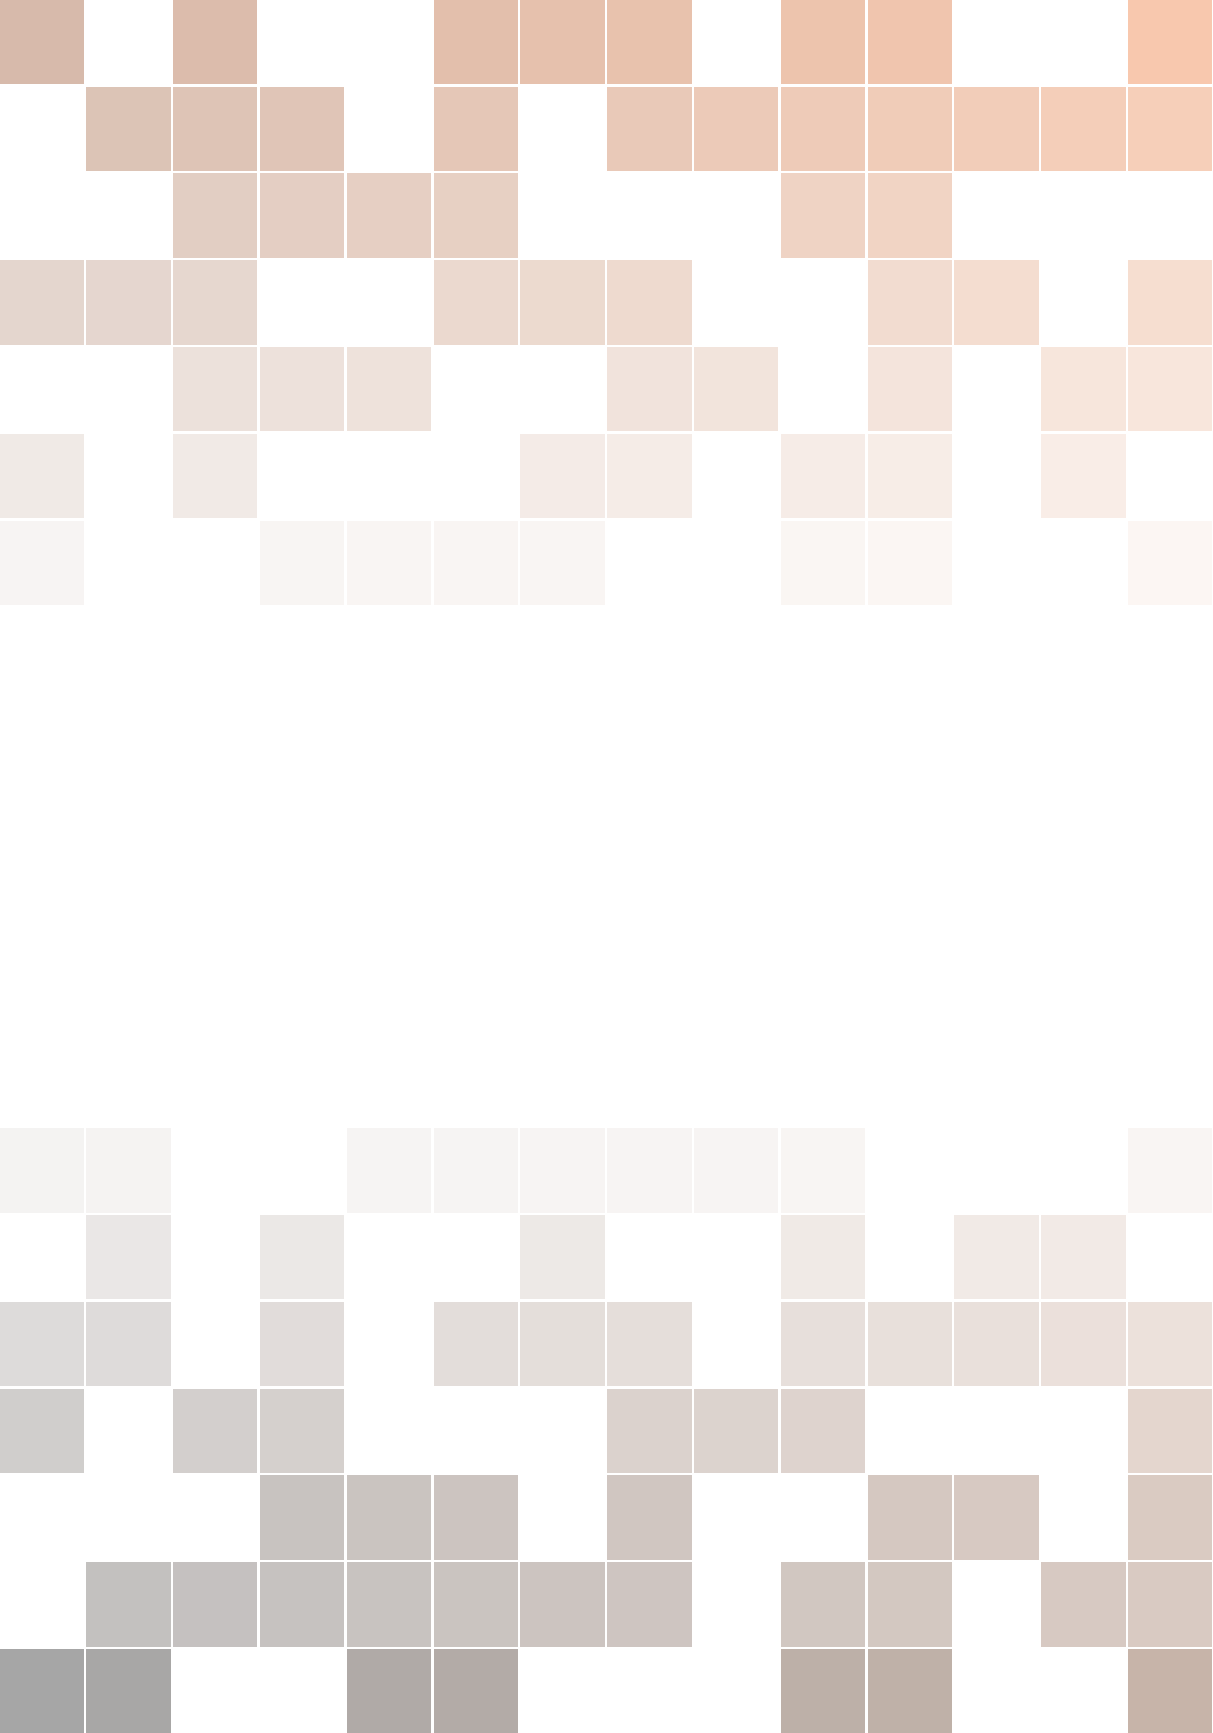
\includegraphics[scale=1]{orange/Pictures/background}}} % Image background
\centering
\vspace*{9cm}
\par\normalfont\fontsize{35}{35}\sffamily\selectfont
\par \slgbooktitle % Book title

\vspace*{1cm}

{\Huge \slgbookauthor}\par % Author name

\vspace{1in}

\fontsize{18}{18}\selectfont\slgbookdate

\endgroup

%----------------------------------------------------------------------------------------
%	COPYRIGHT PAGE
%----------------------------------------------------------------------------------------

\newpage
~\vfill
\thispagestyle{empty}

\noindent \slgbookcopyright\\ % Copyright notice

\noindent \textsc{\slgbookpublisher}\\ % Publisher

\noindent \textsc{\slgbookurl}\\ % URL

\noindent  \slgbookfrontmatter
 
\noindent \textit{\slgbookdate} % Printing/edition date

%----------------------------------------------------------------------------------------
%	TABLE OF CONTENTS
%----------------------------------------------------------------------------------------

\chapterimage{orange/Pictures/chapter_head_1.pdf} % Table of contents heading image

\pagestyle{empty} % No headers

\tableofcontents % Print the table of contents itself

\cleardoublepage % Forces the first chapter to start on an odd page so it's on the right

\pagestyle{fancy} % Print headers again

%% Included from ``textbook.tex''
%%
%% Body of computer forensics textbook
%% Assumes foratting has been set up.

\newif\ifpartone\partonetrue
\newif\ifparttwo\parttwotrue
\newif\ifpartthree\partthreetrue
\newif\ifpartfour\partfourtrue
\newif\ifpartfive\partfivetrue
\newif\ifpartsix\partsixtrue

% Turn off lots
%\parttwofalse
%\partthreefalse
%\partfourfalse
%\partfivefalse
%\partsixfalse

% http://tex.stackexchange.com/questions/17009/how-to-change-code-example-font-in-listings
\lstset{basicstyle=\small\ttfamily,numbers=left,numberstyle=\tiny}
\newcounter{bookpart}\setcounter{bookpart}{0}
\newcommand{\bookpart}[1]{\addtocounter{bookpart}{1}
    \chapter*{Part \arabic{bookpart}:#1 }
    \phantomsection
    \addcontentsline{toc}{chapter}{\textcolor{ocre}{Part \arabic{bookpart}: #1}}
}
\DeclareFieldFormat[inproceedings]{date}{\ifbibliography{\mkbibparens{#1}}{#1}}


\ifpartone
  \bookpart{Task and Tools}
  \chapter{Introduction}\label{ch:introduction}
\setlength{\epigraphwidth}{3in}
\epigraph{Three can keep a secret, if two of them are dead.}{Benjamin
  Franklin}

This book is about finding and exposing data that are \emph{hidden},
\emph{invisible}, or simply \emph{overlooked} in digital systems. When
such data that are privacy sensitive are discovered, the results
frequently include pain, ruined
reputations, financial loss, and even harms to national
security. 

\section{Leaks of Personally Identifiable Information}

Consider these two cases:

\begin{itemize}
\item In April 2011, two software developers discovered that
Apple's iOS~4 operating system kept a database that tracked the movements of every
iPhone and iPad user in a database that was never purged. Worse, the database was copied to the users'
laptop  whenever the phone was backed up using Apple's \emph{iTunes}
program\cite{apple-tracking}. To demonstrate the privacy leak, the developers created an application
exported the data and plot it with Google Maps~(\figref{heatmap}). A
media uproar resulted, forcing 
Apple to make an unplanned release of its operating system that fixed
the bug\cite{apple-tracking-statement}. 

\item Also in April 2011, the UK Parliament posted an Adobe Acrobat Portable
Document Format (PDF) file on its public with sensitive military
information about UK nuclear subs. Although the file had been
redacted and cleared by the British Ministry of Defense,  \emph{The
  Daily Telegraph} discovered that the information had merely been
covered with black boxes, rather than being 
actually removed. A follow-up investigation 
found other PDF files that had improperly redacted on four other UK government
websites\cite{telegraph-april2011-secrets}.
\end{itemize}

\begin{figure}
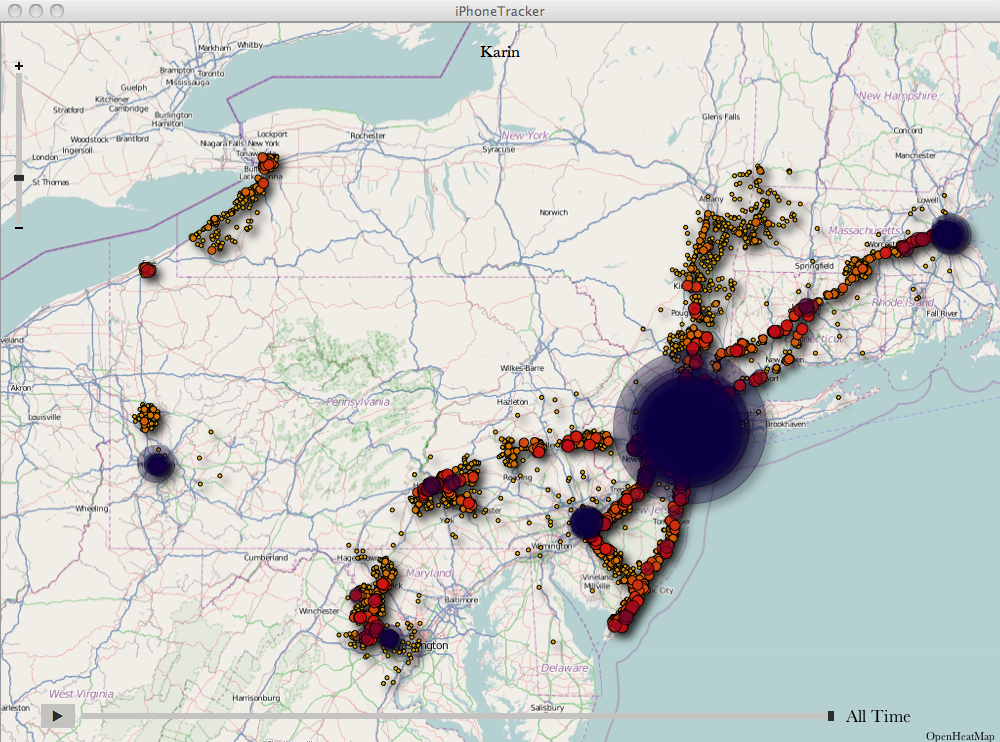
\includegraphics[width=\textwidth]{ch-1/5637893141_ba59f2d989_o.png}
\caption{In April 2011, Pete Warden and Alasdair Allan discovered
that Apple's iOS~4
  operating system recorded the location of nearby Wi-Fi access points
  to aid in geolocation. Due to a bug the database was never
  cleaned. As a result, the database could easily be used to create a
  map of every place that the iPhone had been. \rights{\copyright 2011 John
  Niedermeyer. Licensed under Creative Commons
  Attribution-NonCommercial-ShareAlike 2.0 Generic.}}\label{heatmap}
% http://www.flickr.com/photos/nedward/5637893141
\end{figure}

Hidden data are present in many computer systems. They are stored in
documents, embedded in operating systems, and even encoded and sent over
networks. It's not the \emph{presence} of these data that damages
privacy---it's their inevitable discovery and exploitation.

Most of the technical privacy failures that we know about were not
discovered by the companies that wrote the software in
question. Instead, they were discovered by students,
journalists, and computer ``hackers''---people who looked at the data
and saw something that they thought was worth investigating.

This book teaches approaches for systematically finding privacy
leaks and for documenting what you have found. We call this process
``technical privacy auditing'' because it uses technical tools to find
privacy problems. We believe that many such privacy leaks can be
discovered through straightforward visual inspection and the use of
simple data mining techniques. Once found, many problems can be
avoided with relatively simple software modifications.

Technical privacy auditing can be used by software developers, testers
and customers to evaluate software before it is released or
deployed. The techniques can also be used to examine data before
publishing. The techniques could have been used to prevent the data
leaks by the British MOD or the deployment of privacy-compromising
software to millions of Apple customers.

\subsection{Privacy-leaking Software Bugs}

All kinds of software leaks personal information. Sometimes it is
because the software is improperly used, or because it not designed
to perform a function in a way that preserves privacy. That's what
happened in the case of the British PDFs. Other times the software has
a bug that prevents sensitive information from being properly
removed, as was the case with iOS~4.

Before discovery, these data can be present for a long time without
causing apparent harm. But that doesn't mean that the flaws aren't
known, or aren't being actively exploited. For example, in location
tracking in iOS~4 was widely to digital forensics examiners---the
information had even appeared in a book. The people who knew and made
use of the privacy leak didn't publicize it to the general public
because they didn't want it fixed.  

Over the years a wide variety of software running on many different
kinds of computers have been found to leak private information.  The
violations are usually  
\emph{unintentional}---the programmers who developed the code didn't
create them with the goal of violating their users'
privacy. Nevertheless, the software 
had bugs or usability flaws that caused private information to be
inadvertently retained or distributed. The software problems are
typically so subtle that most users don't realize that their private
information is being compromised. Because the private information
leaked is typically embedded in a form that is invisible or easily
ignored, the flaws can persist for weeks, months, or even years before
they are discovered and fixed.

Software bugs that result in privacy leaks tend to fall into these
broad categories:

\begin{itemize}
\item Failure to destroy privacy-sensitive data when they are no longer needed.
\item Transmission of privacy-sensitive data beyond a protection boundary. 
\item Improper use of encryption.
\end{itemize}

The root cause of many of these bugs is the complexity
of modern information systems. Today's computers are vast, with
gigabytes of storage, tens of thousands of application programs, and
real-time connections to data networks that continually download ever 
more code and data. A typical cell phone with 16 gigabytes of memory can
store literally hundreds of thousands of digital photographs, hours of
video, or months of audio recorded from its internal
microphone. It's very easy for a programmer to overlook some small
piece of storage that may hold some very sensitive piece of
information. 

\subsection{Privacy-leaking Usability Flaws}

Some privacy leaks happen because the user of a program doesn't
realize what the program is doing. There may be several similar
ways for accomplishing a task, one way that eventually leaks
information, one that does not. Poor software design can make these
two approaches seem equivalent.

ways for
acco doesn't realize 
that the software ir what their software is doing. 
doesn't 
Another source of privacy leaks can be software that is *1

Inadvertent privacy leaks aren't limited to government agencies and
major computer manufacturers: many damaging privacy leaks happen
person-to-person because modern computer systems are so
complex. Consider the digital photograph shown in \figref{nsf_hq}. The
original photo showed a readily
identifiable 12-story office building. The photo was cropped to an
eight of its original size, removing much of identifying information. But the cropped
version still contains metadata from the original that
describes the time that the photograph was taken, the fact that it was
taken with an iPhone 4S, and the GPS location of the
photographer to within a few feet. (\figref{nsf_metadata}). JPEG
metadata is discussed in \chapref{ch-jpeg}. The program used to crop
the image didn't the metadata.

\sgraphic{ch-1/nsf_hq}{This photograph of a tree and a few cars contains
  and embedded title and GPS location information.}

\bifigure{ch-1/nsf_hq_exif}{ch-1/nsf_hq_gps}{Metadata from
  \figref{ch-1/nsf_hq}, as displayed by Preview.}


\section{Technical Privacy Auditing}

of ways that private information has been
leaked in modern information systems and shows how you can find 
those leaks using tools that are freely available. 


Privacy leaks such as the hidden information in PDFs and Apple's
unintentional location database are insidious because they are
invisible. They can be present for years in a piece of software that's
used by millions of people. They can be exploited against the interest
of their users. And they are frequently present because nobody looked
deeply at the data or publicized their findings. 

\section{Digital Forensics Tools}

This book teaches approaches for finding leaks of personal information using
digital forensics tools. The previous section gave a brief description
of two kinds of leaks that have happened in recent years. This
section gives a brief introduction to digital forensics, the digital
forensics process (called the ``model'' by practitioners), and how the
leaks described in the first section could have been found using
digital forensics tools.

\subsection{Digital Forensics}

\emph{Digital Forensics} (DF) is a branch of forensic sciences that
involves the investigation digital devices and the data that they
contain for the purpose of proving or disproving a hypothesis about an
event that took place in the past. For example, digital forensics
tools can be used to extract a deleted photograph from a cell phone
and present that photograph in a court of law. The forensic process
can be used to determine whether or not the photograph was taken by the
phone's camera or downloaded to the phone over a network. The process
can also be used to establish when and where the photo was taken.

In recent years the rise of television forensic shows like CSI and
NCIS have presented a somewhat distorted view of DF to
the general public. While the shows accurately convey the important
role that DF has in some cases, television forensics departs from
reality in many important ways. 

On television, forensics is portrayed as being swift and
certain. Forensics software is graphical, easy-to-use, and fast. For
dramatic reasons the forensics team typically has just one or two
specialists that know how to perform a forensics analysis, and they know how
to use \emph{every} tool that the organization has---digital tools,
fingerprints, chemistry, and even nuclear physics. There are typically
no false positives or mismatches in televised forensics. Data that are
overwritten or encrypted can usually be recovered (unless the plot
requires that they not be), and it is nearly impossible to delete
anything. Sadly, such portrayals have caused victims and  juries alike
to have unrealistic expectations about the technical capabilities of
government agencies, something that has come to be known as \emph{the
  CSI Effect}\cite{csi-effect}\cite{beyond-csi-effect}.

Privacy in the digital world would be at considerable risk if digital
forensics truly had such powers: anyone who desired could violate any
secret anywhere. Fortunately, the reality of digital forensics is far
less exciting---and decidedly more pro-privacy.

In the real world, data that are overwritten generally cannot be
recovered, and data that are encrypted usually cannot be
decrypted. This is good news from a privacy perspective: it means that
technical measured, properly applied, really can protect computer
users from accidental data leaks. 

From its inception, DF has served two different purposes:

\begin{enumerate}
\item \textbf{Extracting information from physical devices related to
  a crime.} In the pre-digital age a suspect's address book or
calendar might be entered directly into evidence and handed to the
jury. That's not possible in the digital age, when those materials
might be on a password-protected computer or hidden somewhere inside a
mobile phone. In many cases forensic techniques make it possible to
recover data that have been deleted or hidden but not yet
overwritten. 

\item \textbf{Understanding the details of crimes that are inherently
  digital (``cyber crime'').} DF tools allow the examination of
data from crimes that have no analog in the pre-digital world, such as
breaking in to a computer over a network or planting malware on a
person's mobile phone. In these kinds of cases, DF tools may be the
only way to understand what has happened and attempt to determine the
responsible party. 

\end{enumerate}

DF is powerful because computer systems are windows into the
past. Many digital systems retain vast quantities of
information---either intentionally, in the form of log files and
archives, or inadvertently, as a result of software that does not
cleanly erase memory and files after it runs. As a result, it
is frequently possible for investigators to recover old email
messages, chat logs, Google search terms and other kinds of data
that were created
weeks, months, or even years in the past. Such contemporaneous records
can reveal an individual's state-of-mind or intent \emph{at the time
  the crime was being committed}.

The next section describes how digital forensic tools can be used to
accomplish these goals.

\subsection{The Digital Forensics Model}

Even though every case is different, DF practitioners have developed an
approach to conducting investigations called the 
\emph{digital forensics model}\cite{pollitt:models}. The 
elements of the model include:

\begin{description}
\item[Preparation] Before performing an investigation, those involved
  must prepare themselves by deciding upon the standards and
  procedures that will be followed; receiving the necessary training;
  and obtaining the appropriate equipment and software required for
  investigations. 

  To use the example of the cell phone from above,
  preparation may involve obtaining specialized hardware that can extract the
  memory from a cell phone and practicing one's technique on phones that are not part
  of the investigation.

\item[Collection and Preservation]
  Before data can be analyzed, they   must be removed from the
  device being analyzed and preserved to create a lasting
  record. Without this step, it may not be possible to repeat an
  analysis at a later point in time. 

  In our example, this step might involve the actual extraction of data
  from the cell phone into a single file called a \emph{physical
    image} that records all of the phone's applications, phone data, user data,
  and deleted files. Such a physical image might be 64GB in size or
  even larger.

\item[Examination and Extraction] Working with the preserved data, an
  examiner will explore for any information that might be
  relevant to the investigation at hand. Once that information is
  found, it is extracted and isolated.

  In our example, this step might involve the extraction of each
  digital photograph from the \emph{physical image} and the storage of
  each photograph in its own file. The files might be named according
  to where they were found in the physical image (e.g. 62071808.jpg)
  rather than with the name that they were given by the phone
  (e.g. IMG001.JPG). The examiner might also extract \emph{metadata}
  from each photograph such as the time and GPS coordinates associated
  with each exposure and the serial number of the camera that took the
  photograph. This information might be stored in a separate file for
  each photograph (e.g. 62071808.txt) or might be stored in a single
  spreadsheet for all of the photographs (e.g. jpeg-metadata.xls).

\item[Analysis] Once the specific data being analyzed has been
  extracted, the analyst will construct one or more hypotheses that
  uses the digital evidence to explain possible past activities. A
  hypothesis may draw from multiple digital devices---an email message
  sent from a desktop computer to a cell phone, for example---or the
  hypothesis may incorporate events in the physical world, like a
  power failure or theft. During this phase a good analyst will also
  try to construct alternative hypotheses that are consistent with the
  evidence but which point to different conclusions. 

  In our example, the hypothesis may be that a specific photograph was
  taken with the phone in question. This may be supported by the
  photograph having similar metadata to a photograph taken a few
  minutes earlier or later. An alternative hypothesis may be that the
  photograph was downloaded to the phone over a network.

\item[Reporting and Testimony] Finally, the analyst will
  produce a written report or give testimony in a courtroom.
  Judges and juries can't examine digital evidence for
  themselves---even if they had the training and the technical skills
  to do so, performing their own analysis would be inappropriate:
  their role in the legal process is to evaluate the law, the evidence
  and make a legal determination, not to perform technical
  analysis. Reports and testimony must therefore be 
  \emph{complete}---they must describe the tools and procedures
  that were followed, clearly document what was found, and then
  separately provide the technical interpretation of the
  evidence. 

  In our example, the analyst might prepare a report documenting how
  the phone's contents were copied, the tools that were used to
  extract the photographs and their corresponding metadata, and how
  the evidence is consistent with the analyst's hypothesis. 

\end{description}

The model brings reliability and repeatability to the process, helping
to assure that different examiners working with the same data will
arrive at the same conclusion. 

Because they can look into the past and uncover hidden data, DF tools
are increasingly used beyond the courtroom. Security professionals use
DF tools to analyze network intrusions---not to convict the attacker,
but to understand how the attacker gained access to plug the
hole. Data recovery firms use DF tools to resurrect files from drives
that have been inadvertently formatted or damaged. 

\subsection{A Microscope for finding Personally Identifiable Information (PII) }

Our goal is to use
the model for privacy auditing. We want to detect the presence of
information that is personally identifying or potentially
sensitive. To do this, we'll use DF tools as a kind of digital
microscope. Like a biologist looking for bacteria or other signs of
contamination, if we find sensitive information, we'll know that there is a potential
for a privacy leak.

The term \emph{personally identifiable
  information} (PII) is frequently used as shorthand sensitive
information that should not be disclosed, and we'll use that shorthand
here. The term is unfortunate, however, as not all personally identifiable information is
sensitive and not all sensitive information leaks personally
identifiable information. Nevertheless the term is widely used and
even enshrined in many US laws, so we will use it here as well.

Our basic approach will be to treat privacy auditing as an
experimental science. We will create specially manufactured documents,
computer media and network streams that are likely to contain known
PII. We will then use DF tools to see if we can find the PII that we
have inserted. This will allow us to both understand how the tools
work and how the PII moves through a digital system. Finally, we will
apply the same tools to documents, media and network streams acquired
in the ``wild''---in the digital environment---and see if those wild
samples contain PII. If they do, we have documented a privacy failing.

Others have used DF tools for this purpose. For example, in 2009 the
Inspector General of the United States Department of Defense issued a
report in which forensic software was used to test hard drives leaving
the government service. The IG found that ``DOD Components did not
properly sanitize, document, or fully account for excess unclassified
IT equipment before it was released to other Federal, DOD, or
non-Federal organizations.''\cite{D-2009-104}

Both of the privacy leaking examples at the beginning of this chapter
could have been readily prevented by applying the digital forensics
model:

\begin{enumerate}
\item \textbf{The UK PDF files.} The reports in the British
  newspapers demonstrated  that it didn't take specially trained DF
  practitioners using expensive tools to recover the data from the
  MoD's improperly redacted PDF files. All that was required was a
  copy of Adobe Acrobat Reader. 

  Applying the DF model would have put the MoD in a better position to
  preventing the disclosure in the first place. Starting with proper
  training, the organization would have been better positioned to
  understand the difference between removing sensitive information and
  simply covering it up. After the files were sanitized, forensic tools
  could have been used to search for key words, terms,
  or labels associated with sensitive or restricted information: if
  such keywords were found, the tools could have been used to identify
  the process failings. When the redaction process was corrected and
  re-applied, the tools could then verify that the redaction had been
  completed as expected.

\item \textbf{The Apple Geolocation Database.} Likewise, Warden and Allan didn't
  require special forensic tools to find the covert geolocation
  database that was present in iOS~4. The database was a standard SQLite3
  file, and the file was stored as part of the iPhone ``backup''
  database present on every Macintosh or Windows computer that was
  synched with an iPhone using Apple's iTunes program. The database
  was ready to be found by any privacy professional that did an audit
  of those files, for the simple fact that it was larger that all of
  the other databases in the backup: whereas most of the databases were typically
  10KB to 100KB in size, the geolocation database from some iPhones was
  in the 10MB to 100MB range. The database was so large because it was
  never pruned; it was a privacy violation for the same rason.

  The computer forensics model applied to the iPhone system could have
  readily caught the privacy leak before the iPhone software was
  released to the general public. An important part of the Analysis
  step is to look for and try to explain outliers: the database
  was such an outlier that should have attracted attention. 
\end{enumerate}


\section{Conventions used in this book}
In general this book follows \emph{Wikipedia Manual of
  Style}\footnote{\url{http://en.wikipedia.org/wiki/Wikipedia:Manual_of_Style}}
and specifically the Computer
Science\footnote{\url{http://en.wikipedia.org/wiki/Wikipedia:WikiProject_Computer_science/Manual_of_style}}
  and
  Computing\footnote{\url{http://en.wikipedia.org/wiki/Wikipedia:Manual_of_Style/Computing}}
  sections. Specific conventions useful in understanding this book are
  described below.

\subsection{Fonts}

Text in this book is generally typeset in the serif font that you are
now reading. The fixed-width courier font is used for programs,
computer input and output, as well as for numbers that might
reasonably be expected to be constants in a computer program. Thus,
the Earth is 150 million kilometers (150 Gm) from the sun, but a
traditional disk sector has |512| bytes (|512|~B).

\subsection{Radix}
Numbers are generally assumed to be in base 10 unless otherwise
specified. Binary digits are suffixed with a |b|; octal
is indicated with a leading |0| as in most programming
languages; hexadecimal numbers may be prefixed with |0x| or |\x| or
have a |h| suffix. Unfortunately there are
exceptions that must be inferred from context. For example, hex dumps
and cryptographic hashes are always presented courier as unadorned hexadecimal
digits. Examples are shown in \tabref{nomenclature}.

\begin{table}
\begin{tabular}{cllrl}
     &              &         & Decimal  \\
Base & Nomenclature & Example & Equivalent      & Usage \\
\hline
\hline
2  & Binary      &  |10101111b|& 175            & Text\\
\hline
8  & Octal       &  |0377|     & 255            & Text and code\\
   &             &  |\377|     & 255            & Code\\
\hline
10 & Decimal     &  |1234|     & 1234           & Text and code\\
\hline
16 & Hexadecimal &  |DEADBEEFh|& 3,735,928,559  & text \\
   &             &  |0xFF|     & 255            & Output \\
   &             &  |\xFF|     & 255            & Python code\\
\hline
\hline
\end{tabular}
\caption{Examples of numbers in various bases used in this book.}\label{nomenclature}
\end{table}

\subsection{Units}

Measurements for Natural phenomena discussed in this book are provided
in SI Units (the ``Metric System.'')
Manufactured objects are described in either SI units or
United States customary units (followed by SI approximations), depending on the system of measurements
that was used to design and produce the object. Thus, this book
discusses 5.25-inch (133mm) floppy disks.

\subsection{SI and IEC Multipliers}\label{sec:si-and-iec}
% \note{1MB = 1,000,000 bytes}
% \note{1MiB = 1,048,576 bytes}

Today there are two standards in computing for representing sizes of
files, storage systems, and memory banks: SI (the International System
of Units) decimal prefixes and IEC (International Electrotechnical
Commission) binary prefixes. This situation is confusing because until
recently the SI prefix names \emph{kilo}, \emph{mega} and \emph{giga} were commonly used
for both decimal and binary notation, the specific multiplier presumably
inferred from context. Today there is an effort underway to clarify
usage. 

The confusion dates back to the early days of computing, when the ``K''
and ``M'' prefixes were commonly used to mean 1,024 and 1,048,576
when describing memory systems but 1,000 and 1,000,000 when
describing mass storage systems. The difference stems
from the fact that memory locations are  addressed
with a series of binary address lines, while electro-mechanical drums and
disks are addressed by specifying a head, a track, and then counting
sector numbers: such numbers only map to even powers-of-two when the
number of heads, tracks and sectors are also powers-of-two, and
this is rarely the case due to manufacturing concerns.

For much of computing history the correct sense of Ks and Ms could be
inferred from context and, in any event, the difference between 1000
and 1024 wasn't all that significant. Those in the industry knew that
a megabyte of RAM was really $1024\times1024=1048576$ bytes.

The difference in interpretation became an issue in the 1990s as the
number of people using computers mushroomed fierce pressure to cut
costs hit the storage industry. A storage vendor could truthfully
advertise and sell a ``600 MB''
hard drive that stored 600,000,000 bytes in
precisely 1,171,875 512-byte sectors. There was simply no incentive
for storage vendors to sell such a hard drive that stored
$600\times1024\times1024=629,145,600$ bytes and required 1,228,800
sectors to do so.

A second reason for the standardization effort was the increasing
ridiculousness stemming from computer scientists using
a non-standard system of measurement. Really, why should the K prefix
mean 1024 when describing bytes but 1000 when describing grams?

A third reason for the standardization was the industry's move to
increasingly larger storage systems, resulting in successively larger
divergence between the power-of-two measurement and the corresponding
power-of-ten measurement. This third reason is almost certainly the
reason that binary-based prefixes were proposed in the 1990s---that's
when the need for the prefixes started to become noticable.

The IEC binary prefixes were proposed in 1996\cite{iec:1996}, and
adopted as an international standard in 1999.  In 2006 additional
prefixes were adopted for exbi (Ei=$2^{60}$), zebi (Zi=$2^{70}$) and
yobi (Yi=$2^{80}$)\cite{iec:80000-13:2008}.

Despite this standardization effort, today we live in a somewhat
confusing world in which so-called ``4GB'' DRAM modules 
store precisely 4,294,967,296 bytes
but ``4GB'' microSD cards sold for cell
phones store 4,000,000,000 bytes. Even more confusing, the DRAM
module may have four ($2^{2}$) chips, each storing 1073741824
($2^{30}$) bytes each, while the microSD card may two million flash
pages, each with 4096 bytes of usable storage, but present that
information as precisely 7,812,500 logical 512-byte blocks.  These
differences are the result of different kinds of electronics to access
these storage devices, different kinds of software that use them, and
different economics for producing them. 

It is likely that the IEC binary prefixes will be increasingly popular
over time. This book uses the binary prefixes to describe block size
and sector size, since they are typically multiples of 512 ($2^9$),
but SI decimal prefixes to describe disk sizes, since that is the way
the devices are sold to consumers.

SI decimal prefixes are commonly used to represent SI
quantities. For example, the SI prefix \emph{kilo} multiplies the value that follows by
$10^3$; thus a kilogram (Kg) is
$10^3=1,000$ grams and a kilobyte (KB) is
$10^3=1,000$ bytes. The IEC prefix \emph{kibi} multiples the value following by $2^{10}$. A \emph{kibibyte}
(KiB) is thus $2^{10}=1,024$ bytes. Those two values are similar but
different (see \tabref{si-iec-differences}

This has been proper usage
since 1999 when the IEC adopted standard 60027-2 for binary prefixes.


% http://www.codinghorror.com/blog/2007/09/gigabyte-decimal-vs-binary.html

\newcommand{\WZ}{{\color{white}0}}

\begin{table}
\begin{tabular}{||llr|llr|rl|}
\multicolumn{3}{c}{SI Prefix} & \multicolumn{3}{c}{IEC Prefix} & $\Delta$ & root \\ 
\hline
kilo  & K & $10^{3\WZ} = 1000^1 $ & kibi & Ki & $2^{10} = 1024^1 $& 2\% & Greek root {thousand} \\
\hline
mega  & M & $10^{6\WZ} = 1000^2 $ & mibi & Mi & $2^{20} = 1024^2 $& 5\% & Greek root \emph{megas}, {great}\\
\hline
giga  & G & $10^{9\WZ} = 1000^3 $ & gibi & Gi & $2^{30} = 1024^3 $& 7\% & Greek root for {giant}\\
\hline
tera  & T & $10^{12} = 1000^4$ & tebi & Ti & $2^{40} = 1024^4 $& 10\% & Greek root for {monster}\\
\hline
peta  & P & $10^{15} = 1000^5$ & pebi & Pi & $2^{50} = 1024^5 $& 13\% & Greek root for \emph{penta}, {five}\\
\hline
exa   & E & $10^{18} = 1000^6$ & exbi & Ei & $2^{60} = 1024^6 $& 15\% & Greek root for \emph{hexa}, {six}\\
\hline
zetta & Z & $10^{21} = 1000^7$ & zebi & Zi & $2^{70} = 1024^7 $& 18\% & Mangled Latin root for \emph{septum}, {seven}\\
\hline
yotta & Y & $10^{24} = 1000^8$ & yobi & Yi & $2^{80} = 1024^8 $& 21\% & Mangled Greek root for \emph{octo}, {eight}\\
\hline
\hline
\end{tabular}
\caption{SI and IEC prefixes: amounts, percent differences, and
  linguistic roots.}\label{si-iec-differences}
\end{table}

\section{Other Resources}
\subsection{Books}
\subsection{Articles}

\section{Exercises}
* Open the JPEG and determine the address of where the photographer
was standing. Show your work.



%%  LocalWords:  Alasdair PDFs repeatability

%  \chapter{Technical Privacy Auditing: A Model For Investigations}
\setlength{\epigraphwidth}{3in}
\epigraph{By failing to prepare, you are preparing to fail}{Benjamin Franklin}

This chapter continues the introduction of technical privacy
auditing by introducing the Technical Privacy Auditing Model and
previewing three examples of how the model will be applied to
different kinds of data later in this book.

\section{The Technical Privacy Auditing Model}

\section{Applying the model redacted PDFs}

\section{Applying the model to JPEGs}

\section{Applying the model to network traffic}


\section{Other Investigation Models}

\subsection{The Digital Forensics Model}

Even though every case is different, DF practitioners have developed an
approach to conducting investigations called the 
\emph{digital forensics model}\cite{pollitt:models}. The 
elements of the model include:

\begin{description}
\item[Preparation] Before performing an investigation, those involved
  must prepare themselves by deciding upon the standards and
  procedures that will be followed; receiving the necessary training;
  and obtaining the appropriate equipment and software required for
  investigations. 

  To use the example of the cell phone from above,
  preparation may involve obtaining specialized hardware that can extract the
  memory from a cell phone and practicing one's technique on phones that are not part
  of the investigation.

\item[Collection and Preservation]
  Before data can be analyzed, they   must be removed from the
  device being analyzed and preserved to create a lasting
  record. Without this step, it may not be possible to repeat an
  analysis at a later point in time. 

  In our example, this step might involve the actual extraction of data
  from the cell phone into a single file called a \emph{physical
    image} that records all of the phone's applications, phone data, user data,
  and deleted files. Such a physical image might be 64GB in size or
  even larger.

\item[Examination and Extraction] Working with the preserved data, an
  examiner will explore for any information that might be
  relevant to the investigation at hand. Once that information is
  found, it is extracted and isolated.

  In our example, this step might involve the extraction of each
  digital photograph from the \emph{physical image} and the storage of
  each photograph in its own file. The files might be named according
  to where they were found in the physical image (e.g. 62071808.jpg)
  rather than with the name that they were given by the phone
  (e.g. IMG001.JPG). The examiner might also extract \emph{metadata}
  from each photograph such as the time and GPS coordinates associated
  with each exposure and the serial number of the camera that took the
  photograph. This information might be stored in a separate file for
  each photograph (e.g. 62071808.txt) or might be stored in a single
  spreadsheet for all of the photographs (e.g. jpeg-metadata.xls).

\item[Analysis] Once the specific data being analyzed has been
  extracted, the analyst will construct one or more hypotheses that
  uses the digital evidence to explain possible past activities. A
  hypothesis may draw from multiple digital devices---an email message
  sent from a desktop computer to a cell phone, for example---or the
  hypothesis may incorporate events in the physical world, like a
  power failure or theft. During this phase a good analyst will also
  try to construct alternative hypotheses that are consistent with the
  evidence but which point to different conclusions. 

  In our example, the hypothesis may be that a specific photograph was
  taken with the phone in question. This may be supported by the
  photograph having similar metadata to a photograph taken a few
  minutes earlier or later. An alternative hypothesis may be that the
  photograph was downloaded to the phone over a network.

\item[Reporting and Testimony] Finally, the analyst will
  produce a written report or give testimony in a courtroom.
  Judges and juries can't examine digital evidence for
  themselves---even if they had the training and the technical skills
  to do so, performing their own analysis would be inappropriate:
  their role in the legal process is to evaluate the law, the evidence
  and make a legal determination, not to perform technical
  analysis. Reports and testimony must therefore be 
  \emph{complete}---they must describe the tools and procedures
  that were followed, clearly document what was found, and then
  separately provide the technical interpretation of the
  evidence. 

  In our example, the analyst might prepare a report documenting how
  the phone's contents were copied, the tools that were used to
  extract the photographs and their corresponding metadata, and how
  the evidence is consistent with the analyst's hypothesis. 

\end{description}

The model brings reliability and repeatability to the process, helping
to assure that different examiners working with the same data will
arrive at the same conclusion. 

Because they can look into the past and uncover hidden data, DF tools
are increasingly used beyond the courtroom. Security professionals use
DF tools to analyze network intrusions---not to convict the attacker,
but to understand how the attacker gained access to plug the
hole. Data recovery firms use DF tools to resurrect files from drives
that have been inadvertently formatted or damaged. 

  % investigation models
  % \chapter{How Data are Stored}
As indicated above, while the primary storage system of most computers can be accessed a
byte at a time, secondary storage can only be accessed in
blocks. Secondary storage, in turn, can be divided into two broad
categories:

\begin{description}
\item[Block addressable] storage systems are systems for which any
  block can be individually read or written. Each block in a block
  addressable system is assigned a \emph{logical block address}
  (LBA). 
\item[Streaming] storage systems are those that allow blocks to be
  read or written as part of a sequence. Most streaming systems are
  based on a spool of magnetic or optical tape. New blocks can be
  written to the tape and the tape supports limited operations---for
  example, \emph{rewind}, writing a \emph{mark}, \emph{seeking} to a mark,
   \emph{erasing} and possibly \emph{overwriting}. In general it is
   not possible with a streaming system to reliably overwrite a single
   block---attempts to do so may result in other blocks being damaged
   and rendered unreadable.
\end{description}

Confusingly, although we have used the term \emph{block} exclusively
until now, many vendors use the term \emph{sector} to describe blocks
that are written to spinning discs. (The term is presumably comes from
the fact that data was originally stored in concentric circles on a spinning platter
and in bands on a rotating magnetic drum. Thus, each block occupied a
sector of a circle.) Until the mid 2000s most mass storage systems
used blocks (sectors) that were 512 bytes in size. Since then vendors
have moved to systems that use 4096-byte blocks internally, although
many still give the appearance of using 512-byte sectors to provide
for software compatibility. 

\subsection{Drives, Hard Drives, Solid State Drives}

\subsection{Write Blockers}

Removable media such as floppy disks, tapes and storage cartridges
used in the 1990s generally had some kind of \emph{write-protect}
switch or tab that could be used to prevent inadvertant alternation or
overwriting of evidence. Hard drives of the time had no such
facility. To overcome this deficiency the industry invented
\emph{write-blockers}, a device that can be inserted inline between a
hard drive and a computer system. A typical write blocker might have a
male and a female ATA-33 connector; the female connector plugs into
the hard drive's male ATA-33 connector, while the blocker's male
connector plugs into a cable that connects to the host computer.

Write blockers allow examination of subject data without fear of
inadvertently modifying the contents---provided that the write blocker
works properly. A problem with the concept of write blockers is that
the only real specification of what these devices should do was their
name---that is, they should block modification of data on the hard
drive.  But there
are two ways to do this. One is to literally block the commands that
alter data, a task that requires a clear enumeration of all such
commands. An alternative (and somewhat safer) strategy is to only pass
those commands that are known \emph{not} to alter
data\cite{dfrws2006:JamesLyle}. Both of these approaches
implicitly assume that the only way data is altered on the drive is
through the execution of commands, and this is not actually the
case. For example, the S.M.A.R.T. counters inside modern drives that
track the number of seconds the drive is powered up will continue to
advance even when a write-blocker is in place.

\subsection{Disk Imaging and Disk Images}
Two problems that are not solved by write blockers. First, the
digital evidence still resides on the original media, which is a
mechanical device and subject to failure. Second, most legal systems
allow for both parties to have access to evidence. Both of these
problems can be overcome by making a sector-for-sector copy of the
disk, a process called \emph{disk imaging}.

The most basic way to image a disk is to copy every sector onto
another disk of the manufacturer and model number. Such a disk is
called a \emph{mirror copy} or \emph{mirror volume}. Once the copy is made, the subject disk
can be kept sealed in an evidence locker and the mirror volume can be
used for forensic analysis. 

A difficulty in making a mirror copy is that it may not be possible to
obtain a drive of the exact make and model number. Fortunately, it is
only necessary for the copy disk to be larger than the original. The
sectors between the end of the original disk and the copy disk should
be ignored.

[Figure: original disk, copy, and the section to ignore.]

\subsection{Inaccessible Information}

TK - DCO and HPA

TK - SMART information

 % How data are stored
  \chapter{Understanding Disks, Files and File Systems}
As a computer user you are familiar with files. This chapter looks in
detail at how files are stored on \emph{mass storage devices} such as
hard drives and camera cards (``drives.''). It shows how two popular file systems
(FAT and NTFS) store information in files and directories, and how the
information on the media changes when the user attempts to delete a
file.

As we will see, many file systems retain a significant amount of
potentially sensitive information even after a file is deleted. This
retention isn't \emph{inherent}, but it is \emph{common}. 
System designers could design computer systems that erase all traces of
sensitive data when files are deleted, but they generally don't, because
overwriting deleted data has real costs in terms of performance,
battery consumption, and increased code complexity.

Computer forensic tools such as Sleuth
Kit\footnote{http://sleuthkit.org/sleuthkit/} take advantage of this
\emph{residual information} that's left behind after a file deletion
and make it possible to recover deleted files---provided that the data
have not been overwritten by new information. Thus, the ability to
recover files depends not just on the specific software that
was used, but how the drive used \emph{after} the file or files were
deleted.  \index{Sleuth Kit} \index{residual information}

In order to understand how information is recovered,
we'll need to learn how files and directories are stored in the first
place. We'll also learn how to construct an experiment that you can
use to determine if data is left behind or not. That's useful for
analyzing new file systems that are not implemented by existing
forensic tools.

Tools used in this chapter:
\begin{itemize}
\item Hex dump tool
\item Python
\item SleuthKit 
\end{itemize}

\section{Disks, Sectors, Files and File Systems}
This section describes how files are stored on mass storage devices
such as flash cards, solid state drives and spinning hard drives. 


\subsection{Mass Storage Systems: Organization and Addressing}

\index{sector}
Mass storage systems don't store files. Instead, they store blocks of
bytes, traditionally called \emph{sectors} (as in a \emph{sector of a
  circle}). Sectors are typically
sized as a power of 2. In the 1990s most hard drives had a sector
size of 512~B; modern drives (both SSD and HD) have a block size of
4~KiB. Compact Discs (CDs) and Digital Video Discs (DVDs) have a sector size of 2048~B.
A 1~TB drive therefore has approximately 250 million 4~KiB
blocks. (For an explanation as to why blocks are sized in powers of
two but hard drive storage is not, see \secvref{sec:si-and-iec}.)

\twofigures{.55\textwidth}{ch-fs/1024px-Seagate_ST33232A_hard_disk_inner_view.jpg}{Inner
  view of a Seagate 3.5 inches hard disk drive 
  manufactured in 1998. This drive has 3 platters, 6
  physical read/write heads, and a total storage of 3,227~MB. (photo: Eric
  Gaba, Wikimedia Commons)}{.4\textwidth}{ch-fs/sdcard}{Two SanDisk SD
  Cards manufactured in 2003. Each card has 1,000~MB of solid state
  storage. (photo: Simson L.\ Garfinkel)}

Each block on the media is referenced by a distinct number
called a \emph{logical block address} (LBA). The drives discussed in
this chapter are
\emph{random access}, meaning that the computer can read or write any
block in any order, although it is invariably faster to read or write
blocks multiple blocks at a time in numeric order.
\index{LBA|see {Logical Block Address}}
\index{Logical Block Address}

Users don't see blocks of bytes when they take an SD card out of a
camera and try to read the contents on a laptop: they see folders
and files. The \emph{file system} is the part of the computer's
operating system that implements the \emph{file abstraction layer},
taking the \emph{file names} used by people and application programs,
and mapping them to specific numbered blocks of data on the mass
storage device. 
Confusingly, the phrase \emph{file system} is also used to
describe a specific set of sectors on a specific piece of
media. 
 
The file system provides an API that allows program to read and write
the contents of files, which ultimately results in the contents of
specific disk sectors being copied into regions of memory specified by
the application. File systems also provide a facility for grouping
multiple files into \emph{folders} or
\emph{directories}. Finally there are provisions for creating and
deleting files, renaming files, moving files from one directory to
another, creating and deleting directories, and so on. Each of these
changes to the file system structure must eventually be reflected by
changes to sectors on the mass storage device.

Most modern computers define a \emph{file} to be a sequence of zero or more
bytes. In practice files can have additional properties such as one or
more \emph{file names}, a \emph{creation date}, a \emph{last modification date},
\emph{last access data}, and so on. Many systems also have a way of
specifying the file's \emph{type}, or the kind of information that is
stored inside the file. On Windows and Unix the file type is
inferred from the file's extension---a file named
\emph{FOOBAR.JPG} is assumed to be a JPEG digital image. But using
extension to infer file type is not universal: the HTTP protocol sends
the MIME file type along with the file length in the HTTP header when
a file is downloaded over the web.

Mass storage systems can only read or write complete blocks, so the
file system may also have to buffer data between the application
program and the drive. This means that information on the disk can
also be found in the computer's memory. This can become a privacy
problem, as  data can remain in memory  after they are erased from
a drive.


\subsection{Historical Background}
In the 1950s engineers at IBM devised a method for storing digital
information on a rotating ferromagnetic disc. As the disk spun a pair
of read/write heads (one for the top side, one for the under side)
could be moved to one of several set distances from the center of the
disk. Each surface of the disk was thus divided into a set of stacked
concentric tracks, called \emph{cylinders}, each divided into a set of
adjacent sectors. The original IBM 350 (\figref{ibm-305}) had 50 spinning 24-inch that
could store a total of 5 million bits, whereas a modern
hard drive might have two spinning platters and store a 2~TB, but the
underlying principal remains the same. 


\sgraphic{ch-fs/BRL61-IBM_305_RAMAC}{An IBM 305 RAMAC computer system at U.S. Army Red River
  Arsenal, with two IBM 350 disk drives in the foreground. Each IBM
  350 consisted of fifty 24-inch diameter disks, creating 100 recording
  surfaces, each with 100 tracks, each track holding 100 5-bit
  characters, for a total storage of 5~Mb.\cite{ibm-350}\label{ibm-305}} 

 \twofigures{.45\textwidth}{ch-fs/Cylinder_Head_Sector}{The structure
   of a traditional hard drive consists of multiple platters, 
   each with two read/write heads. The surface of each
   platter is divided into concentric tracks, with each track divided
   into a number of sectors. The set of all tracks on all of the
   platters  the same distance from the center hole is
   referred to as a \emph{cylinder}, allowing each sector to be identified by
   a Cylinder, Head, Sector (CHS) address. Modern hard drives store more sectors on
 the outer tracks than the inner tracks so that data is recorded at a
 constant areal density. These drives refer to each
 sector by a Logical Block Address (LBA), rather than by
 CHS.}{.45\textwidth}{ch-fs/cd}{The data on an optical disc is arranged
   as a series of blocks in a single spiral, with information recorded
   at a constant linear density. Blocks are referred to by their
   Logical Block Address. CD-ROM (Compact Disc Read Only Memory) media
   is manufactured with its data; CD-R (Compact Disc-Recordable) can
   be recorded by users, but only once; CD-RW (Compact
  Disc-ReWritable) media can be erased and re-recorded.\textbf{TK: Draw Spiral}}


While disks turned out to be cost-effective  for storing large
amounts of information, they require that information to be broken up
into identically sized blocks, each stored at a
specific location. Requiring users to deal with this level of detail
would be unworkable. Instead, computers provide facilities for
assigning labels to sequences of sectors. The first use of the early
disk drives was to replace cardboard file boxes of punched cards that
were used to programs and data, so it was only natural that those
sequences of sectors were called \emph{files} as well. We use the same
terminology today.

Early disk systems enumerated each sector with the specific cylinder,
head and sector (CHS) that was used to access it. This approach gave
computer designers a great deal of control over the precise storage of
data, but also greatly complicated the design of software. The biggest
complication was something called \emph{bad block management}\index{bad block management}---how
the computer responded when disk sectors did not perform reliably.
Computer systems were made faster and more reliable by moving bad
block management into the drive itself. The interface was made
simpler by having the computer refer to blocks by a single
\emph{logical block address} (LBA), generally an integer greater than
or equal to 0, and allowing the drive to map the LBA to a specific
location on the media. 

Remember that files are an \emph{abstraction} created to make it
easier to manage data. There is nothing inherent in the design of
computers, operating systems or mass storage devices that requires the
use of files. Indeed, the raw storage offered by mass storage devices
can also be used for virtual memory \emph{backing store} or to store the raw
contents of a database. These kind of non-file system uses were common
in the 1990s. Today, however, virtual memory and databases are
typically stored in files, thanks to advances both in processor speed
and software engineering. 

\index{Cylinder Head Sector}
\index{CHS|see {Cylinder Head Sector}}
\index{Logical Block Address}
\index{LBA|see {Logical Block Address}}

\subsection{FAT---A simple file system from the 1980s}
FAT12, FAT16 and FAT32 are simple file systems developed by Microsoft
in the 1980s for use with the original IBM PC computers. The
definitive specification of the Microsoft's various implementations of
the FAT file system is the \emph{Microsoft Extensible Firmware
  Initiative FAT32 File System Specification}, rev. 1.03, Dec 6,
2000\cite{microsoft-efi}.\footnote{There are actually more than a dozen
  versions of the FAT file system, as different operating systems have
  implemented it slightly differently. The Wikipedia article
  \url{https://en.wikipedia.org/wiki/File_Allocation_Table} does an
  excellent job summarizing many of the differences between the major
  versions.} What follows is a summary of the more
significant elements that you will need to understand basic FAT file systems.

``FAT'' is
an acronym that stands for File Allocation Table. The ``table'' is an
array of integers (either 12-bit, 16-bit or 32-bit) which the file
system uses to keep track of which sectors hold user data and which
are free. In this section we summarize the major features of FAT. We
will focus our attention on FAT16, a version that is used in many
digital cameras.

The FAT disk can be divided into four distinct regions:
\begin{itemize}
\item \emph{The reserved sectors}, located at the beginning of the file
  system. The most important reserved sector is the BIOS Parameter
  Block (BPB) which is defined to be the first sector of the file system.
\item \emph{The FAT region,} which contains one or more copies of the
  File Allocation Table. 
\item \emph{The root directory region}, which stores the root
  directory. FAT stores each directory as
  a list of 32-byte directory records. FAT12 and FAT16 drives store have a
  fixed-size root directory that is located directly after the
  FAT. FAT32 drives use a variable-length root directory that
  typically starts after the FAT but can then move to other parts of
  the disk.
\item \emph{The data region}, which holds \emph{data
  clusters} that are used to store both user data and
  directory contents. Each cluster consists of one  or more
  sequential 512-byte sectors. 
\end{itemize}

These regions are shown graphically in \figref{fig:fat16} for the
FAT16 file system of a 128MB SD camera card taken from a Canon
PowerShot SX 260 HS camera.

\begin{figure}
\caption{A conceptual view of a FAT16 file system. Each box
  represents one or more disk sectors.\label{fig:fat16}}
\begin{center}
% Draw grid that looks like a FAT16 volume
\newcommand{\dbox}[3]{\draw[#1] (#2 -.4, #3 - .4) rectangle (#2 + .4, #3 + .4);}
\newcommand{\Dbox}[3]{\fill[#1] (#2 -.4, #3 - .4) rectangle (#2 + .4, #3 + .4);}
\begin{tikzpicture}[x=.25cm,y=.25cm]
\foreach \y in {1,...,8} {
  \foreach \x in {1,...,40} {
    \dbox{}{\x}{\y}
  }
}
  \Dbox{color=red}{1}{8}  
  \foreach \x in {3,...,4} { \Dbox{color=blue}{\x}{8}  }
  \foreach \x in {5,...,6} { \Dbox{color=green}{\x}{8}  }
  \foreach \x in {7,...,8} { \Dbox{color=pink}{\x}{8}  }
                           { \Dbox{color=cyan}{9}{8} }
  \foreach \x in {11,...,30} { \Dbox{color=yellow}{\x}{8}  }
  \foreach \x in {31,...,40} { \Dbox{color=purple}{\x}{8}  }
  \foreach \x in {1,...,15} { \Dbox{color=purple}{\x}{7}  }

{\small
  \Dbox{color=red}{1}{-1}  ; \node [right] at (1,-1) {MBR};
  \Dbox{color=blue}{6}{-1} ; \node [right] at (6,-1) {FAT1};
  \Dbox{color=green}{11}{-1} ; \node [right] at (11,-1) {FAT2};
  \Dbox{color=pink}{16}{-1}  ; \node [right] at (16,-1) {Root};  
  \Dbox{color=cyan}{20}{-1}  ; \node [right] at (20,-1) {Subdirs};
  \Dbox{color=yellow}{26}{-1} ; \node [right] at (26,-1) {File \#1};
  \Dbox{color=purple}{32}{-1} ; \node [right] at (32,-1) {File \#2};
  \dbox{}{38}{-1} ; \node [right] at (38,-1) {Free};
}
\end{tikzpicture}
\renewcommand*{\dbox}{}
\renewcommand*{\Dbox}{}

\end{center}
\end{figure}

To read the contents of a file on a FAT media the operating system
must decode the structures that make up the file system. This starts
when the computer reads the file system's BPB
to learn the size of the FAT, the size of the root directory, the
cluster size, and other file system parameters. 

Next, the computer will read the first copy of the FAT into
memory. (If there is an error attempting to read the first FAT, it
tries to read the second, and so on.) As mentioned above, the FAT is
an array of 12, 16 or 32-bit integers.  The integers in the FAT don't refer to individual blocks. Instead,
they refer to \emph{clusters}, where a  \emph{cluster} is a contiguous
set of 1, 2, 4, 8 or more disk blocks. The \emph{cluster size} is
file system parameter that is specified when the disk is
formatted. Therefore, a FAT32 file system with a cluster size of 512
(1 sector) has
a maximum file system size of $512\times2{32}=2\textrm{GiB}$, while a
cluster size of 4096 allows for a file system up to 16~GiB. 

The FAT array serves two purposes: it identifies the \emph{allocation
  status} of each cluster---that is, whether the cluster is free and
available for use or if it holds user data. If it does hold user data,
the array tells the operating system how to find each successful
cluster that makes up the file.  For example, if a file occupies
clusters 10 and 11, then slot \#10 in the FAT will contain an |11| and
slot \#11 will contain a special marker that indicates there are no
more clusters in the chain.

Finally, the computer will read the root directory. As mentioned
above, each FAT directory consists of a sequence of 32-byte
records. FAT12 and FAT16 file systems required that file names have a
maximum of 8 characters, a period, and then a 3-character extension,
producing a so-called ``8.3 filename.'' \tabref{table:fatdir} shows
the major elements of the FAT directory entry. FAT32 directory entries
use multiple 32 bytes entries in a row to hold Unicode ``long file
name'' entries that are concatenated together and form an alias for
the short 8.3 file name. The creation and interpretation of long file
names is beyond the scope of this chapter.


\begin{table}
\begin{minipage}{\textwidth}
\caption{The 32 bytes of the FAT directory entry. The first byte
  contains either the beginning of the short file name or a flag
  indicating that the entry is the last or that the entry has been
  deleted and should be ignored. (From Wikipedia, \url{https://en.wikipedia.org/wiki/File\_Allocation\_Table}.)}\label{table:fatdir}
\begin{center}
\begin{tabular}{lll}
\hline
Offset & Length & Description \\
\hline
|00h| & |8| & Short file name (padded with spaces) \\
      & |1| & |00h| -- This is the last entry, and it is available \\
      & |1| & |E5h| -- This entry is deleted; ignore it \\
\hline
|08h| & |3| & Short file extension \\
\hline
|0Bh| & |2| & File attributes and flags\\
\hline
|0Dh| & |1| & Create time miliseconds times 10\\
\hline
|0Eh| & |2| & Create time (bits 15--11:hours; 10--5:minutes; 4--0:seconds)\\
\hline
|10h| & |2| & Create date (bits 15--9:year; bits 8--5:month; bits 4--0: day)\\
\hline
|12h| & |2| & Access date \\
\hline
|14h| & |2| & FAT12 and FAT16: Extended Attributes handle\\

      &     & FAT32: Top 16 bits of cluster with start of file\\
\hline
|16h| & |2| & last write time\\
\hline
|18h| & |2| & last write date\\
\hline
|1Ah| & |2| & Bottom 16 bits of start cluster\\
\hline
|1Ch| & |4| & Size of file\\
\hline
\end{tabular}
\end{center}
\end{minipage}
\end{table}





\subsection{Partitioning and Volume Management}

Although a file system can be stored directly on a drive, with the
first block of the drive being used to store the first block of the
file system, this is not commonly done. Instead, the first 
block of the drive is typically used to store a \emph{disk label} and  \emph{partition
  table} that provides the storage media with a unique identifier and describes the
locations of the file systems that the media contains. Advantages of
this approach include:
\begin{itemize}
\item A single physical device can contain multiple partitions, each
  with its own file system.
\item Partitions can identify specific regions of the disk as reserved
  or encrypted, so that the operating system doesn't inadvertently
  damage them.
\item The device label allows the operating system reference the media
  by name, rather than by location such as the interface or bus. This
  allows computer hardware to be reconfigured without having to update
  operating system configuration.
\end{itemize}

One of the most commonly used partitioning schemes are the
\emph{Master Boot Record} (MBR) format, originally created in 1982 for
the IBM PC/XT and used with minor revisions ever since.

The MBR occupies the first sector of a hard drive used on most
Windows-based computers. When the computer starts up the Basic
Input/Output System (BIOS) loads these 512 bytes into the start of
memory and jumps to location 0. Typically the MBR contains a short
program that loads more sectors from the hard drive into memory and
runs them; this second boot loader loads the operating system and runs
it.

\begin{table}
\begin{minipage}{\textwidth}
\caption{Structure of the Master Boot Record. ({\small from Wikipedia, \url{http://en.wikipedia.org/wiki/Master_boot_record}})}\label{mbr}
\begin{tabular}{|>{\tt}c|>{\tt}c|c|c|c|}
\hline
\multicolumn{2}{|c|}{\bf Address} & \multicolumn{2}{c|}{}                              & \\
\cline{1-2} \bf Hex & \bf Dec         & \multicolumn{2}{c|}{\multirow{-2}{*}{\bf Description}} & \multirow{-2}{*}{\bf Size in bytes}\\
\hline
+000h & +0   & \multicolumn{2}{c|}{Bootstrap code; extended information} & |446| \\
\hline
\hline
+1BEh & +446 & \multicolumn{2}{c|}{Partition entry \#1} & |16| \\
\hline
+1CEh & +462 & \multicolumn{2}{c|}{Partition entry \#2} & |16| \\
\hline
+1DEh & +478 & \multicolumn{2}{c|}{Partition entry \#3} & |16| \\
\hline
+1EEh & +494 & \multicolumn{2}{c|}{Partition entry \#4} & |16| \\
\hline
+1FEh & +510 & |55h| & & \\
\cline{1-3}
+1FFh & +511 & |AAh| & \multirow{-2}{*}{Boot Signature} & \multirow{-2}{*}{2} \\
\hline
\hline
\multicolumn{4}{|r|}{\textbf{Total size: $\bf 446 + (4\times16) + 2 $}} & \textbf{512}\\
\hline
\end{tabular}
\end{minipage}
\end{table}


\begin{table}
\caption{Structure of the 16-byte partition
  entry. {\small(From Wikipedia, \url{http://en.wikipedia.org/wiki/Master_boot_record})}}\label{mbr:partition}
\begin{tabular}{|>{\tt}c|>{\tt}c|l|}
\hline
\textrm{Offset} & \textrm{Length} & Description \\
\hline
+0h & 1 & Status; |80h|:active; |00h|: inactive \\
+1h & 3 & CHS address of first sector in partition (not used on modern systems) \\
+4h & 1 & Partition Type Code \\
+5h & 3 & CHS address of last sector in partition (not used on modern systems)\\
+8h & 4 & LBA address of first sector in partition \\
+Ch & 4 & Number of sectors in partition \\
\hline
+0h & 16 & Total number of bytes in entry \\
\hline
\hline
\end{tabular}
\end{table}

The basic MBR (\tabref{mbr}) provides for four partitions, each
described by a 16-byte partition entry record. The record includes a
byte indicating if the corresponding partition is active or not, the
start of the partition and the partition's length.  Originally the
start and end were encoded as a 3-byte CHS (Cylinder, Head, Sector)
triplet. Today the CHS entries are ignored and the partition is
described with a pair of 32-bit LE numbers conveying the Logical Block
Address (LBA) of each partition's first block and a block
count. Because blocks are assumed to be 512 bytes, this scheme allows
for a maximum media size of $512 \times 2^{32}=2\textrm{TiB}$ in
storage.

The MBR was first introduced by
IBM PC DOS 2.0 in 1983. Since then there have been at least six different
versions of the MBR
used\footnote{\url{http://en.wikipedia.org/wiki/Master_boot_record}}. ALl
of the MBRs store bootstrap code
at location |0|, place the first four partition entries starting at location
|1BEh|, and have a boot signature in the last two blocks of the
sector. This consistency provides for backwards compatibility,
allowing each generation of disk utilities and BIOS drivers to make
sense of whatever data they might find on a mass storage device.
Modern computers use a new partitioning scheme called the GUID
Partition Table
(GPT)\footnote{\url{http://en.wikipedia.org/wiki/GUID_Partition_Table}},
but even these systems include something called a ``Protective MBR''
that allocates the entire drive to a partition of type |EEh|. As its
name implies, this partition protects the GPT disk in the event that
the user attempts to mount it on a system that does not understand GPT
partitioning: instead of inadvertently overwriting the GPT partition,
the non-GPT system will leave it alone, since the entire media is in
use by a partition type that the non-GPT system does not understand.


\subsection{Flash Memory, Solid State Drives, and the Flash Translation Layer}

Flash memory storage was introduced to consumers in the 1990s as a
data storage system for digital cameras, digital audio players, and
personal digital assistants. Flash storage is
similar to magnetic storage systems in that flash is \emph{non-volatile} and block
addressable. It is different in that blocks are grouped into
\emph{pages} that be explicitly erased
as a set before the individual blocks can be rewritten, and each block
experiences \emph{wear} each time it is erased, and as a result each
block can only be rewritten finite number of times before it
fails. Typically this limit is between a thousand and a hundred
thousand rewrites. Despite these limitations, flash has
steadily grown in popularity because of its physical durability (there
are no moving parts), its speed of access (no seek time), and its
steadily increasing storage capacities.

Because file systems like FAT tend to repeatedly rewrite a small
number of sectors used for file system metadata (e.g. the file
allocation table), these file systems cannot be used directly with
flash storage: doing so would cause the ``hot'' blocks holding the
rapidly changing metadata to wear out, since the metadata needs to be
updated each time a file is created or deleted. In a digital camera
application, for example, blocks devoted to the File Allocation Table
would be destroyed after only a few thousand photographs had been
taken, creating a media with an unacceptably short lifespan.

Modern flash storage systems get around this problem with a technique
called wear leveling. The flash storage device implements a
\emph{Flash Translation Layer} that maps the logical block address
viewed by the operating system to the physical flash page used by the
storage device. Each time a block is rewritten, the new data are
written to a new physical locations. Periodically
the FTL writes a new \emph{translation table} to the device with the
mapping. As a result, writes to hot blocks such as the FAT are cycled
through the physical storage device, and instead of being able to
handle thousands of rewrites, the flash device can accommodate 
thousands of billions. 

Although in theory it is possible to access to physical storage of a
flash device, in practice the FTL hides the physical layer and allows
access only to the logical blocks.

\subsection{Encrypting File Systems}

Adding to the complexity of the is \emph{encryption}, which can be
applied at nearly any location between the user and the storage
media. Using encryption provides a significant layer of security: with
encryption, the data on the storage system can be accessed but not
understood unless the appropriate decryption key is available.

Encryption is very flexible. It can be within the storage device itself (as in the case of an
encrypting hard drive), in the operating system's disk driver, in the logical volume
management system, in the file system, or at the application level. 

Encryption is discussed in \chapref{ch:encryption}.


\subsection{Putting it all together: A 128~MB FAT16 Disk Image}
In this section we will explore the contents of an SD camera card
created in 2013 with a Canon PowerShot SX260~HS camera. The card is called NPS-2009-CANON2.

To create the data for this section, we started with a 128MB camera
card and cleared every addressable sector by overwriting that sector's
content with NULL bytes. We did this by inserting it into a Linux
computer. Inserting the card caused Linux to create two devices in the
|/dev| file system:

\begin{tabular}{ll}
|/dev/sdb| & Virtual device for the entire physical volume \\
|/dev/sdb1| & Virtual device for the first partition \\
\end{tabular}


We then unmounted the FAT16 file system and wiped the physical volume
with these commands:

\begin{code}
$ (@ \sl{sudo umount /dev/sdb1} @) 
$ (@ \sl{sudo dd if=/dev/zero of=/dev/sdb} @)
\end{code}
%$

This |dd| command is conceptually similar to the program in Listing\ref{clear.py}.

You can do this
easily with the program in \figref{overwrite}.

\lstinputlisting[caption=\textbf{clear.py}: A simple program to clear a disk.]{ch-fs/clear.py}\label{clear.py}

After the card was cleared, we put it into the PowerShot, initialized
the card, took two photos, deleted the first with the camera, and then
removed the card and put it back in the same Linux computer. Finally
we used the |dd| command a second time to copy the raw blocks into a
disk file, creating a \emph{disk image}:\footnote{You can download that file
from \url{http://digitalcorpora.org/corp/nps/nps-2013-canon1/nps-2013-canon1.raw}}

\begin{code}
$ (@ \hl{sudo umount /dev/sdb1} @)
$ (@ \hl{sudo dd if=/dev/sdb of=nps-2013-canon1.raw conv=noerror,sync} @)
\end{code} 

The |dd| command copies blocks of data from the input file (\emph{if=})
to the output file (\emph{of=}). Two conversion options are
specified: \emph{noerror} tells the \emph{dd} command to continue even
if it encounters an error, and \emph{sync} tells the program to keep
the output stream synchronized with the input stream in the event of
an error by writing blocks filled with NULLs.  Notice that each time we unmounted the file system but imaged the
entire drive. In this way we get the partition table and the slack
space before the beginning of the first file system.  


\subsection{Viewing canon1's MBR}

\figref{fig:fat16l} shows a conceptual view of
canon1's storage. The card has a Master Boot Record in its
first sector (block |0|) which has two slots: slot 1 is an unallocated
region between blocks |0| and |96| (including, somewhat confusingly, the
master boot record itself). Slot |2| is a DOS FAT16 file system that
occupies blocks |97| through |250879|. The FAT file system contains its own
structures, including a \emph{Boot Sector Structure} that describes the
file system, a \emph{root directory}, \emph{subdirectories},
\emph{files}, and finally a \emph{file allocation table} that both
describes which sectors belong to which file and indicates which
sectors are free and available for new files. We'll discuss each of
those in the following section.


You can display the contents of the MBR by viewing a hex dump of the
first sector:

\begin{code}
$ (@ \hl{xxd -a -len 512 nps-2013-canon1.raw} @)
0000000: 0000 0000 0000 0000 0000 0000 0000 0000  ................
*
00001b0: 0000 0000 0000 0000 0000 0000 0000 0003  ................
00001c0: 0200 0607 e0d3 6100 0000 9fd3 0300 0000  ......a.........
00001d0: 0000 0000 0000 0000 0000 0000 0000 0000  ................
00001e0: 0000 0000 0000 0000 0000 0000 0000 0000  ................
00001f0: 0000 0000 0000 0000 0000 0000 0000 55aa  ..............U.
$ 
\end{code}

The |-a| option tells the |xxd| command to suppress identical lines
from the first line (that is, lines that contain 16 NULLs), the \texttt{-len~512} tells the command to only display the first 512 bytes of the
file, and |nps-2013-canon1.raw| is the file name.

Decoding this output is not difficult but can be time consuming. Instead of
manually attacking the hex values, it is more effective to write a
program that does this work for you. Listing~\ref{mbrdecode} the start
of such a program in Python. This program  will open
up the disk image, read the sector into memory, and then print the
fields. 

\begin{figure}
\lstinputlisting[caption=The start of a python program to display the
  Master Boot Record.]{ch-fs/mbrdecode.py}\label{mbrdecode}
\end{figure}

Finally, you can view the contents of the MBR using the SleuthKit's |mmls| command:

\begin{code}
$ (@ \hl{mmls /corp/nps/drives/nps-2013-canon1/nps-2013-canon1.raw} @)
DOS Partition Table
Offset Sector: 0
Units are in 512-byte sectors

     Slot    Start        End          Length       Description
00:  Meta    0000000000   0000000000   0000000001   Primary Table (#0)
01:  -----   0000000000   0000000096   0000000097   Unallocated
02:  00:00   0000000097   0000250879   0000250783   DOS FAT16 (0x06)
$ 
\end{code}

Use the \texttt{-h} option to display all of the options that your
version of the |mmls| command supports.


The first block of a FAT file system contains a \emph{Boot Sector
  Structure} that describes the file system's parameters, including
the sector size, the cluster size, the number of reserved sectors, the
number of File Allocation Tables, and so on. The layout of this
structure is described in Microsoft's FAT specification; you can also
find it in the SleuthKit file |tsk3/fs/tsk_fs.h|\footnote{The current
  version of this file can be found at \url{https://github.com/sleuthkit/sleuthkit/blob/master/tsk3/fs/tsk_fs.h}.}. The first
few lines of the SleuthKit structure are show in \figref{BSS}.

\begin{lstlisting}[caption={The first few bytes of the Boot Sector
      Structure, the first sector of a FAT file system. From
      Sleuthkit's \texttt{tsk\_fs.h}.\label{BSS}}]
/*
 * Boot Sector Structure for TSK_FS_INFO_TYPE_FAT_12,
 * TSK_FS_INFO_TYPE_FAT_16, and TSK_FS_INFO_TYPE_FAT_32
 */
    typedef struct {
        uint8_t f1[3];
        char oemname[8];
        uint8_t ssize[2];       /* sector size in bytes */
        uint8_t csize;          /* cluster size in sectors */
        uint8_t reserved[2];    /* number of reserved sectors for boot sectors */
        uint8_t numfat;         /* Number of FATs */
        uint8_t numroot[2];     /* Number of Root dentries */
        uint8_t sectors16[2];   /* number of sectors in FS */
        uint8_t f2[1];
        uint8_t sectperfat16[2];        /* size of FAT */
        uint8_t f3[4];
        uint8_t prevsect[4];    /* number of sectors before FS partition */
        uint8_t sectors32[4];   /* 32-bit value of number of FS sectors */

        /* The following are different for fat12/fat16 and fat32 */
        ...
\end{lstlisting}

Because the FAT file system begins in sector |97|, the number |97|
must be added to all internal references. Typically this is done in
the device driver, since the device driver must be aware of the disk
partitioning scheme.   

From the parameters stored at sector |97| it is possible to
calculation the location of each of the parts mentioned above.  The
first fat is stored at an offset specified by |reserved|, which must
be interpreted as a 16-bit LE number.  The space allocated by the FATs
is equal to the number of FATs times the number of sectors per
FAT. The number of sectors taken up by the root directory is equal to
the number of root entries times 32 divided by the number of bytes per
sector. Finally there is the data region, which is the start of
cluster \#2. (Cluster numbers 0 and 1 are reserved.)

\section{Exercise: Windows - Creating and Testing FAT32 Disks}

This exercise is designed to help you understand how file systems
store information and the opportunities for retaining
privacy-sensitive information that is not visible to the user. 

This exercise will be done with a \emph{virtual disk}. Like a physical
mass storage device, a virtual disk consists of a set of numbered data
blocks. But instead of storing those blocks directly in on a mass
storage device, the blocks are stored in another file. The operating
system treats the virtual disk like a physical drive: it can be
formatted, files can be copied to it, and so on. But we can also
access the underlying file that holds the virtual disk. This makes it
easier to inspect the individual data blocks.

We will use the Windows |DISKPART| command to create and manage virtual
disks. |DISKPART| is a command-line tool that needs to run as
Administrator.

We will be using these commands:

\begin{tabular}{>{\tt}ll}
\hline
help partition & shows partition command available\\
create vdisk & Creates a virtual disk \\
list disk & Shows available disks \\
list vdisk & Shows detailed information about the available VDisks\\
list partition & Shows available partitions \\
\hline
\end{tabular}

We will create a text file on the virtual disk that has a sensitive file
name and file contents. Next we will take a screen shot and save it on
the computer's hard drive as a JPEG. We will then delete the text file
and empty the trash. Finally we will inspect the disk image and see if
we can find the text file and the screen shot.


\begin{enumerate}


\item Click the Start button, type |diskpart| into the search field,
and click on the |diskpart| program icon.
\item The User Account Control will ask you to verify that you want to
run the DiskPart, a program that can make ``changes to the computer.''
Click ``Yes.''  The |diskpart.exe| window should appear.
\item If you haven't done so already, right-click on the window's
titlebar and select ``Properties.'' Click on the Layout tab and change
the ``Screen Buffer Size'' to 9999. This will allow you to scroll
backwards and see the entire history of your DISKPART session.
\item Type |help| to see the list of commands that the DISKPART
command supports. You may need to make the window larger.

\item Create a 16MB virtual disk with the command:

\begin{code}
DISKPART> (@ \hl{create vdisk file="C:\textbackslash{}disk1.vhd" maximum=16} @)
\end{code}

\item Attach the disk you just created:
\begin{code}
DISKPART> (@ \hl{attach vdisk} @)
\end{code}

\item Verify that the disk is attached:
\begin{code}
DISKPART> (@ \hl{list disk} @)
...
DISKPART> (@ \hl{list vdisk} @)
\end{code}

\item Now we need to create a partition, assign a letter to that
partition, and format the drive. We will call this drive K: and format
it with FAT. 
\begin{code}
DISKPART> (@ \hl{create partition primary} @)
DISKPART> (@ \hl{assign letter=k} @)
DISKPART> (@ \hl{format fs=fat label="WORK"} @)
\end{code}
\end{enumerate}

At this point we have a 16MB virtual disk attached to the computer as
drive K:. The drive's contents are stored in the file |C:\disk1.vhd|.

Lastly, we want to put a file on this disk. For test purposes we are
going to use a small file with a distinctive file name and file
contents.

\begin{enumerate}[resume]
\item Run the windows NotePad program by clicking the Start program,
typing ``Notepad'' into the search field, and clicking on the icon.

\item Type this text into the document:  ``The phone number is
202-555-1212.'' You can use your own phone number and add additional
information if you wish.

\item Select ``File/Save As'' and save the file on the WORK (K:) drive
with the name ``file-name-example-0001.txt''. 

\item Close the Notepad program.

\item Now we will detach the virtual disk:

\begin{code}
DISKPART> (@ \hl{detach vdisk} @)
\end{code}

\end{enumerate}

\subsection{Looking for the files}
The 

\section{Working with Disk Images}

Today there are three fundamental kinds of forensic data:

\begin{itemize}
\item Disk Images
\item Memory Images
\item Packets intercepted on a network.
\end{itemize}

Most research to date has been done with Disk images. Most data is
stored on disk, and most forensic investigations have been for the
purpose of finding information that is on a disk (such as in the case
of a child pornography investigation), or in trying to understand
information left behind on a disk (for example, after an intrusion or
malware incident.

It is also common to find the other kinds of information on disk
images. Memory is frequently stored on disk images from swapping
(e.g. PAGEFILE.SYS on Windows) or system hibernation
(HIBER.SYS). Packets are found on image files when the disks were used
to store the results of a network interception.

Working with image files can consists of these activities:


\begin{itemize}
\item Copying the data from the source drive into the image file, a
  process called \emph{drive imaging}.
\item Computing the checksum of the disk image.
\item Validating the copy against the original.
\item Creating a digital signature for the disk image.
\item Self-validating the copy.
\item Making backup copies of the disk image, and validating the integrity
  of the backups.
\item Converting the disk image into a form that can be used by your
  forensic tool
\end{itemize}.

On the \url{digitalcorpora.org} website there are several disk images with
which you can work. We're going to do our initial work with the image
nps-2009-canon2-gen6. This image is usually stored in the directory
/corp/drives/nps/nps-2009-canon2/.

The nps-2009-canon2 disk images are a series of images created with a
Canon digital camera and a 32MB SD card. First the card was
\emph{cleared} using |dd| on a Linux computer. The card was then
inserted into the digital camera, a series of photos were taken, and
the card was removed and imaged. The card was put back into the
camera, some of the photos were deleted, and new photos were
taken. This process was repeated five times, creating a total of six
disk images, nps-2009-canon2-gen1 through nps-2009-canon2-gen6.

The SD card contained 60,800 512-byte sectors, for a total of
31,129,600 bytes (30,400 KiB).

For each disk image four files are distributed:

   .raw -- a raw disk image that's 31,129,600 bytes in length
   .E01 -- An EnCase E01 file of the disk image
   .xml -- A digital forensics XML file describing the files resident
           in the disk image.


It is customary in digital forensics to use cryptographic hashes to
verify the integrity of a disk image. When the disk is first imaged
the hash is recorded in a secure manner (typically written in in
investigator's notebook). From that point forward, the image can be
manually validated by recomputing the hash and comparing it to the
original recording.

The hash of a raw file can be easily calculated the ``openssl''
command:

\begin{Verbatim}
$ openssl md5 /corp/drives/nps/nps-2009-canon2/nps-2009-canon2-gen6.raw
MD5(/corp/drives/nps/nps-2009-canon2/nps-2009-canon2-gen6.raw)=750b509d8fbed37a5213480aaccfdc61
$ 
\end{Verbatim}

You can't calculate the hash of an E01 file in this manner,
however, because these files contain additional metadata that is not
part of the disk image.  Both of these formats also store hash codes
directly in the disk image. This allows you to \emph{validate} the
contents of a disk image with a command that calculates the hash by
examining the data and comparing it with the stored value. 

\subsection{E01 files}
You can use the ewfinfo command to view the metadata information of a
disk image:

\begin{Verbatim}
% ewfinfo /corp/drives/nps/nps-2009-canon2/nps-2009-canon2-gen6.E01 
ewfinfo 20090927 (libewf 20090927, libuna 20090901, libbfio 20090927, zlib 1.2.3, libcrypto 0.9.8)

Acquiry information
Acquiry date:Mon Apr 12 08:12:32 2010
System date:Mon Apr 12 08:12:32 2010
Operating system used:Darwin
Software version used:20090927
Password:N/A

EWF information
File format:EnCase 6
Sectors per chunk:64
Error granularity:64
Compression type:no compression
GUID:dc032794-bef0-2c45-8ede-8cc01ed31683

Media information
Media type:removable disk
Is physical:no
Bytes per sector:512
Amount of sectors:60800
Media size:29 MiB (31129600 bytes)

Digest hash information
MD5:750b509d8fbed37a5213480aaccfdc61

% 
\end{Verbatim}


You can verify the contents of an E01 file using the ewfverify
command:

%% BEGIN NO FILL
\begin{Verbatim}
$ ewfverify /corp/drives/nps/nps-2009-canon2/nps-2009-canon2-gen6.E01 
ewfverify 20090927 (libewf 20090927, libuna 20090901, libbfio
20090927, zlib 1.2.3, libcrypto 0.9.8)

Verify started at: Mon Jun  7 14:20:20 2010

This could take a while.

Status: at 0%.
        verified 32 KiB (32768 bytes) of total 29 MiB (31129600 bytes).

...

Status: at 100%.
        verified 29 MiB (31129600 bytes) of total 29 MiB (31129600 bytes).

Verify completed at: Mon Jun  7 14:20:20 2010

Read: 29 MiB (31129600 bytes) in 0 second(s).

MD5 hash stored in file:750b509d8fbed37a5213480aaccfdc61
MD5 hash calculated over data:750b509d8fbed37a5213480aaccfdc61

ewfverify: SUCCESS
$ 
\end{Verbatim}
%% END NO FILL




\subsection{Exercises}
\begin{itemize}
\item Download an install the following programs in this order:
\begin{itemize}
\item   libewf
\item  sleuthkit
\end{itemize}
\item Download nps-2009-canon2-gen6.e01 and nps-2009-canon2-gen6.raw
\item Verify the SHA1 of each file. Verify the RAW with the openSSL
  command and make sure that it matches what is in this book. Use the
  ewfverify and afverify commands to verify that the hash codes stored
  in the E01 files match the computed values.
\item Convert the RAW file to an E01 files. Notice that the
  files are different than the distribution E01 files.
\item Verify your converted files.
\item Convert the distribution E01 files back to raw files and
  use the Unix |cmp| command to show that the resulting files match
  the distribution raw file.
\end{itemize}


\section{Going Deeper}
\subsection{File Systems of Interest}
There are a many different kinds of file systems in use on
modern computer systems:
\begin{description}
\item[Disk file systems] organize files and directories on
  block-oriented storage systems. 
\item[Memory file systems] implement a file abstraction in
  memory. Such systems can provide for increased performance when
  compared to using a conventional file system on a simulated block
  device. One of the most common examples of a memory file system is tmpfs\cite{Snyder90tmpfs:a}.
\item[Distributed file systems] allow a computer to access
  information on remote servers as if it is stored
  locally. Distributed file systems are forensically interesting
  because many use local storage to cache information from the remote
  servers. Analyzing local storage can therefore give clues as to what
  was accessed remotely, and when it was accessed. Examples of
  distributed file systems include Sun's Network File System
  (NFS)\cite{Sandberg85designand,Pawlowski00thenfs} and Microsoft's
  Common Internet File System (CIFS)\cite{ms-cifs}.
\item[Virtual file systems] use the file and directory abstraction to
  make it easy to access other information. For example, the Linux
  |/dev| file system is used to access devices through the file
  system, the |/sys| file system is used to access features within
  the system kernel, and the |/net| file system accesses the
  automounter. Virtual file systems are not typically of interest in
  MEDEX because they do not leave residual information on a storage
  device. However, virtual file systems are relevant in malware
  analysis and intrusion response.
\end{description}

As this chapter is written, the following file systems are of general
interest. The number after each file system is date that the file
system became made generally usable:
\begin{description}
\item[FAT12, FAT16 and FAT32 (1980)] file systems developed by Microsoft for use with
  DOS and early versions of Windows. 
  
\item[HFS, HFS+ (1985)] the Hierarchical File System, developed by Apple
  Computer and introduced with the first Macintosh hard
  drive. Whereas most file systems of the time used tables and arrays to store
  information, HFS and HFS+ use b-trees.
\item[NTFS (1993)] the New Technology File System, developed by
  Microsoft for use with Windows NT. 
\item[EXT2/3/4 (1993)] The extended file system, developed for use with Linux systems.
\item[exFAT (2007)] a modification of the FAT file system designed to
  support large files and optimized for use on flash drives.
\item[YAFFS, YAFFS2 (2002)] ``Yet another flash file system,'' a file
  system specifically designed for use with NAND flash chips found in
  cell phones. Unlike other file systems, YAFFS2 specifically adapts
  to the requirement that flash pages be cleared before they can be
  re-written. It also handles wear-leveling and garbage collection.
  YAFFS2 gained popularity through its use in Android, although it is
  increasingly being replaced through the use of proprietary flash
  translation layers (FTLs).
\end{description}

SleuthKit version 4.1 provides read-only support for all of the file
systems listed above. Read-write support for the file systems is
inconsistent, with most operating systems supporting FAT and NTFS,
but support for others being inconsistent.

Confusingly, the phrase \emph{file system} is used ambiguously to
describe both the organization of data on a mass storage device and
the code that implements the file abstraction. Thus, are multiple FAT
implementations, only some of which are authored by
Microsoft. Different file system implementations are supposed to be
mutually compatible, but because of the complexity inherent in
creasing a file system implementation, incompatibilities inevitability
emerge.

Any computational storage device or storage abstraction can be used to
virtualize and contain any other storage device. That is, a file can
be stored in a file system, but a file system can also be created and
stored inside a file (this is essentially what a disk image is). For
example, it is possible to create a USB drive that boots a copy of
Linux but also functions under Windows: The Linux EXT file system is
stored inside a rather large file in an outer FAT32 file system.

\subsection{Books}
\subsection{Articles}
\subsection{Web Sites}
\url{http://www.pjrc.com/tech/8051/ide/fat32.html}
\subsection{Wikipedia}
As of this writing, the following wikipedia pages provide excellent
insight to the concepts mentioned in this chapter:

\begin{description}
\item[\href{http://en.wikipedia.org/wiki/Copy-on-write}{Copy-on-write}]
\item[\href{http://en.wikipedia.org/wiki/Logical_Unit_Number}{Logical
    Unit Number}] Something about the LUN
\item[\href{http://en.wikipedia.org/wiki/Logical_volume_management}{Logical
    Volume Management}]
\item[\href{http://en.wikipedia.org/wiki/Snapshot_(computer_storage)}{Snapshot
    (Computer Storage)}]
\end{description}

\section{Terminology}
\sgraphic{art/diskpart-1}{The Windows diskpart command is used to create and
  manage physical and virtual disks.}


Allocated

Blocks

Carving

Clusters

Deleted

File Allocation Table

Free List

inode

Hard Link

Symbolic Link

Master File Table

Overwritten

TRIM Command

Undelete

Unlink

\section{Exercises---Operating Systems}
This problem set assumes that you have read the draft ``Finding Hidden Data
in File Systems'' chapter of \emph{Technical Privacy Auditing with
  Computer Forensics Tools}

\begin{enumerate}
\item Download canon1\footnote{\url{http://digitalcorpora.org/corp/nps/nps-2013-canon1/nps-2013-canon1.raw}} and show a hex dump of the
  images' first sector.
\item Draw a box around hex bytes in the dump that
  correspond to the first slot in the partition table.
\item Run \texttt{mbrdecode.py} (\ref{mbrdecode}) on Canon1 and provide the results.
\item The first block of Canon1's FAT16 partition contains a Boot
  Sector Structure. Extend \texttt{mbrdecode.py} to read this block
  and print the fields. 
\item Further extend \texttt{mbrdecode.py} to print the contents of the root
  directory.  You will do this by:
\begin{enumerate}
  \item Determining the location and length of the root directory
    from the BSS.
  \item Reading the root directory into a buffer.
  \item Creating a function that takes a buffer and prints each
    directory entry that the buffer contains.  This function will
    operate by stepping through the buffer 32 bytes at a time.
\end{enumerate}  

\item In order to work with files it is necessary to read the File
  allocation table. Using the information you learned in the previous
  step, provide the sector numbers where the FAT starts and stops.
\end{enumerate}

\noindent   Recall that sectors on a FAT volume used to hold user data are
  called \emph{clusters};  each cluster may consist of one or
  more sectors (blocks). Each file can therefore be referred to by the
  number of the cluster where the first byte of file data is
  stored. The FAT array for each cluster contains a pointer to the
  location of the next cluster or a special value indicating there are
  no more data clusters. Each file is therefore described by a linked
  list of cluster numbers, and all of the linked lists for all of the
  files are stored within the fAT.

\begin{enumerate}[resume]
\item Modify the \texttt{mbrdecode.py} program to read the
  entire FAT into an integer array. 
\end{enumerate}
  
\noindent  The remainder of these problems work with two
  files. File \#517 is the
  directory \verb|\DCIM\111___06\| while File \#1030 is the JPEG image
  \verb|IMG_0126.JPG| in that directory.

\begin{enumerate}[resume]
\item  Once you have modified \texttt{mbrdecode.py} to read the entire FAT
  into memory, modify it further to print all of the cluster numbers 
  associated with File \#517. Provide a list of the clusters.

\item Provide a list of the clusters associated with File \#1030.

\item Now that you have a list of data clusters, you can read the
  contents of the files and decode them!  Read File \#517 into a
  buffer and print its contents using the function you wrote that
  decodes file directories. Provide this output and explain each entry.

\item Read File \#1030 and store the results in a file on your host
  computer called \emph{FILE1030.jpg}. Show the contents of that file graphically.

\end{enumerate}
  
\noindent Extra credit:


\begin{enumerate}[resume]
\item Write a program that starts at the root
  directory and recursively lists the name, modification date, and
  size of every file on the disk.
\item Create a virtual disk using the instructions in the chapter. Put
  a few files on the disk and delete a few of them. Read the directory
  and explain which files can be recovered with file recovery
  utilities. Write a file recovery utility and try to recover one or
  more of the deleted files.
\end{enumerate}



\section{Exercises}

\begin{enumerate}
\item Download GEN1 (nps-2009-canon2-gen1.raw) and show a hex dump of the
  images' first sector.
\item Draw a box around hex bytes in the dump that
  correspond to the first slot in the partition table.
\item Show a hex dump of the GEN1 Boot Sector Structure.
\item Run the \texttt{mbrdecode.py} program shown in the chapter on
  GEN1 and provide the results.
\item Extend \texttt{mbrdecode.py} to decode and print all of the
  fields in the Boot Sector Structure. You will do this by:
\begin{enumerate}
  \item Determining the block number in which the BSS resides. (Hint:
    it's the first block of the partition.)
  \item Reading the block into a buffer.
  \item Using \texttt{struct.unpack} to decode the buffer. (You
  can do this in a single statement or with a series of statements as
  we do in the Listing.)
  \item Printing each value. 
\end{enumerate}


\item Extend \texttt{mbrdecode.py} to print the contents of the root
  directory.  You will do this by:
\begin{enumerate}
  \item Determining the location and length of the root directory
    from the BSS.
  \item Reading the root directory into a buffer.
  \item Creating a function that takes a buffer and prints each
    directory entry that the buffer contains. 
\end{enumerate}  

\item In order to work with files it is necessary to read the File
  allocation table. Using the information you learned in the previous
  step, provide the sector numbers where the FAT starts and stops.

\item Modify the \texttt{mbrdecode.py} program to read the
  entire FAT into an integer array. 

  Recall that sectors on a FAT volume used to hold user data are
  called \emph{clusters};  each cluster may consist of one or
  more sectors (blocks). Each file can therefore be referred to by the
  number of the cluster where the first byte of file data is
  stored. The FAT array for each cluster contains a pointer to the
  location of the next cluster or a special value indicating there are
  no more data clusters. Each file is therefore described by a linked
  list of cluster numbers, and all of the linked lists for all of the
  files are stored within the fAT.

  For the remainder of this problem set we will be working with two
  files. File \#517 is the
  directory \verb|\DCIM\100CANON\| while File \#1029 is the JPEG image
  \verb|IMG_0001.JPG| in that directory.

  Once you have modified \texttt{mbrdecode.py} to read the entire FAT
  into memory, modify it further to print all of the cluster numbers 
  associated with File \#517. Provide a list of the clusters.

\item Provide a list of the clusters associated with File \#1029.

\item Now that you have a list of data clusters, you can read the
  contents of the files and decode them!  Read File \#517 into a
  buffer and print its contents using the function you wrote that
  decodes file directories. Provide this output.

\item Read File \#1029 and store the results in a file on your host
  computer called \emph{FILE1029.jpg}. Show the contents of that file.

\end{enumerate}
  
Extra credit:


\begin{enumerate}
\item Write a program that starts at the root
  directory and recursively lists the name, modification date, and
  size of every file on the disk.
\item Create a virtual disk using the instructions in the chapter. Put
  a few files on the disk and delete a few of them. Read the directory
  and explain which files can be recovered with file recovery
  utilities. Write a file recovery utility and try to recover one or
  more of the deleted files.
\end{enumerate}



% LocalWords:  virtualize repurpose

  \chapter{What Data Look Like}

Sometimes you can spot data leakage by simply opening a file with an
ordinary utility, as we did in the last chapter when we used Apple's
Preview application to read geolocation data hidden inside a JPEG. 

Other times the leakage may be less obvious.  The software developers
know that the information is present but don't think that it's
relevant, and people who are in a position to know that the leakage is
relevant don't have the technical ability to determine that it's
present.

This chapter starts with instructions for creating a file that has hidden information
(\secref{sec:make-pdf}). We'll save the file in two ways, as a Rich
Text file (RTF) and as a Portable Document Format (PDF) file. Then
we'll look at the data the file contains using a variety of
techniques, including the raw bytes, a a \emph{hex dump}
(\secref{sec:hex-dumps}), and by extracting the printable strings
(\secref{sec:strings}). 

In order to understand what the hex dump and extracted strings
actually mean, we'll need to see how information such as 
(\secref{sec:numbers}) and letters (\secref{sec:letters}) are 
stored inside a computer's memory or in a file.  Much of this chapter is similar to
what might be covered at the start of a course on computer
architecture. But whereas an architecture course is primarily
concerned with computation and data in motion, this chapter is
concerned with understanding data at rest.

\section{Creating a File with ``Hidden'' text}\label{sec:make-pdf}

\figref{ch-what/textedit_hidden_1} shows how to create a simple file that
contains hidden data using Apple's TextEdit application.\footnote{The
  same set of steps will work with Libre Office or Microsoft Word. We
  use TextEdit here because the resulting RTF and PDF files are the
  simplest.}
 Start by
opening the TextEdit application, type the text, select the word ``Hidden'' and
change the background (highlight) color of the text from ``none'' to
``black.'' (The text background control is the box that looks like this:
\includegraphics[height=1.5ex]{ch-what/textedit_highlight_control}).

Save two copies of the file, one in the Rich Text Format (RTF) in file
a called |hidden.rtf|, the second as an Adobe Portable Document Format
(PDF) file in a file named |hidden.pdf|. (You can use
the same approach with other word processors, but the resulting PDF
file is typically more complicated) 


\bifigure{ch-what/textedit_hidden_1}{ch-what/textedit_hidden_2}{Constructing a PDF with
  hidden text by selecting the text in a word processor (left) and
  then setting the highlight color to black (right).}

The file |hidden.rtf| is seven lines long and has just 297 bytes; that
file's contents appear in \lstref{hidden.rtf}. The file |hidden.pdf|, in
contrast, is 8304 bytes long. If the file's contents were printed here
they would look like a confusing jumble of letters, numbers, and
obscure symbols that would fill four pages. Such jumbled output is 
sometimes referred to as \emph{garbage}, and more properly termed
\emph{binary data} to distinguish it from the printable text that
makes up |hidden.rtf|. 

\sgraphic{ch-what/textedit_hidden-more}{The file {\tt hidden.pdf} viewed with the program \emph{less} running inside the Macintosh Terminal program.}

\lstinputlisting[caption=hidden.rtf,label=hidden.rtf]{ch-what/textedit_hidden.rtf}

\subsection{Viewing a text file}
\subsection{Viewing a binary file}

Attempt to view the file |hidden.pdf| with the
Unix program \emph{less} and you'll be warned:

\begin{code}
$ (@ more hidden.pdf @)
"hidden.pdf" may be a binary file. See it anyway?
\end{code}
%$

Type ``y'' and you'll see results similar to
\figref{ch-what/textedit_hidden-more}. The rest of this chapter explains what
this display means.

\section{Bits, Bytes, and Memory}\label{sec:numbers}
The \emph{bit} is the fundamental unit of storage on digital computers. Bits
have two states. Typically we call these |0| and |1|, but they can be any
two values (e.g. true/false, yes/no or up/down). This book 
uses the values |0| and |1| for bits. (The word \emph{bit} is a contraction of the words \emph{binary digit}.)

An ordered group of 4 bits is called a \emph{nibble}. Each bit can be
a |0| or a |1|, creating 16 possible different values. Note
that $2^4=16$. It is conventional to use the digits 0 through 9 to
number the first 10 possible nibble values, and use the letters A
through F to number the next six, as shown in \figref{nibble}. By
convention computer users call this notation \emph{hexadecimal},
although it's also called Base 16.

To avoid confusion between decimal and binary notation, this book will
always suffix binary numbers with a ``b''. Hexadecimal values have a
``h'' suffix. Some programming languages prefix hexadecimal strings
with a |\x| or |0x|. 

% \marginpar{There are 10 kinds of people in the world. Those who know binary, and those who don't.}


\begin{figure}
\begin{tabular}{>{\tt}c>{\tt}cc>{\tt}cl}
\textrm{binary} & \textrm{octal} & decimal & \textrm{hexadecimal} & english \\
\hline
0000b & 000 & 0 & 0h & zero \\
0001b & 001 & 1 & 1h & one \\
0010b & 002 & 2 & 2h & two \\
0011b & 003 & 3 & 3h & three \\
0100b & 004 & 4 & 4h & four \\
0101b & 005 & 5 & 5h & five \\
0110b & 006 & 6 & 6h & six \\
0111b & 007 & 7 & 7h & seven \\
1000b & 010 & 8 & 8h & eight \\
1001b & 011 & 9 & 9h & nine \\
1010b & 012 & 10& Ah & ten \\
1011b & 013 & 11& Bh & eleven \\
1100b & 014 & 12& Ch & twelve \\
1101b & 015 & 13& Dh & thirteen \\
1110b & 016 & 14& Eh & fourteen \\
1111b & 017 & 15& Fh & fifteen \\
\hline
\end{tabular}
\caption{A nibble is an ordered collection of 4 bits. Each bit can be
  a 0 or 1, so a nibble has $2^4=16$ possible values. This table shows
  the values of a nibble represented in binary, octal, decimal hexadecimal and English.}\label{nibble}
\end{figure}

Modern computers operate on 8 bits at a time, a unit called a
\emph{byte}. Because each bit in the byte can be a |0| or a |1|, and
because the bits are ordered, the byte can represent the values
\texttt{00000000b} through \texttt{11111111b} --- creating a
total of $2^8=256$ possible different values. This book will normally treat
bytes as unsigned integers in the range 0 to 255, but that is just a
convention; the Java programming language treats bytes as signed
integers in the range $-128$ to 127. It's also common to use present
the value of a byte in hexadecimal notation, with the range |00|
through |FF|.

\subsection{Registers}

Computers use groups of bytes to represent larger numbers. Two bytes
can represent 65,536 different values. Here are some examples:

\begin{tabular}{c>{\tt}c}
decimal & \textrm{binary} \\
\hline
0      & 00000000b 00000000b \\
255    & 00000000b 11111111b \\
256    & 00000001b 00000000b \\
65,280 & 11111111b 00000000b \\
65,535 & 11111111b 11111111b \\
\hline
\end{tabular}

Modern computers use registers in a variety of sizes. Many low-cost
embedded systems use 8-bit and 16-bit registers, most cell phones use
32-bit registers, and modern laptops, desktops and servers use
64-bit registers. There are also 80-bit registers used for some kinds
of scientific computing where both high resolution and high speed are required.

\subsection{Memory}

In the example above, the right-hand byte is called the \emph{least
  significant byte} and represents the bits $2^0$ through $2^7$; the
left-hand byte  called the \emph{most
significant byte}; it represents the binary values $2^8$ through
$2^{15}$. 

Because most computer memories are arranged as an array of bytes,
there are two ways to store these 16-bit values at a particular memory
location. 


% http://en.wikipedia.org/wiki/Single-precision_floating-point_format

Larger numbers Two bytes can be grouped together, allowing values between 0 and
65,535 to be represented. Four bytes

\section{Text, ASCII and Unicode}\label{sec:letters}

Modern computers do not work with bits directly, but use sequences of
8 bits called bytes. This sequence can represent
$2\times2\times2\times2\times2\times2\times2\times2=2^8=256$ distinct
values. The meaning assigned to these values generally depends on the
context. A few examples are shown in \tabref{tab:8bits}. The ASCII
codes represent NULL (no data is sent), SOH (Start Of Heading---the
beginning of a data header), and DEL (delete). NULL is a holdover from
the days of synchronous terminals, when there needed to be a constant
flow of data down all links: sending all 0s (NUL) meant that the data
should be ignored. DEL was chosen as delete when characters were
punched on paper tape and cards: in the event of an error, the
operator could backspace the punch and punch holes across the entire
line, causing the computer to ignore the value. We shall return
to the question of representation in \chapref{chap:unicode}.

\begin{table}
\begin{tabular}{cccccccc|c|c|c|c}
\multicolumn{8}{r}{                       Term:}  & unsigned char & signed char & ASCII \\
\multicolumn{8}{r}{                       Range:} & 0--255      & -128--127 & NULL--DEL\\
\cline{9-11}\multicolumn{8}{c}{Bits}                          &        &               &             &          \\
$2^7$ & $2^6$ & $2^5$ & $2^4$ & $2^3$ & $2^2$ & $2^1$ & $2^0$  &        &               &             &          \\
  128 &    64 &   32 &    16 &     8 &     4 &     2 &     1  &        &               &             &          \\
\hline
    0 &     0 &    0 &     0 &     0 &     0 &     0 &     0 &            0  &            0  &   NULL     \\
    0 &     0 &    0 &     0 &     0 &     0 &     0 &     1 &            1  &            1  &   SOH      \\
    0 &     1 &    0 &     0 &     0 &     0 &     0 &     1 &           65  &           65  &   A        \\
    0 &     1 &    1 &     0 &     0 &     0 &     0 &     1 &           96  &           65  &   a        \\
    0 &     1 &    1 &     1 &     1 &     1 &     1 &     1 &           127 &          127  &   DEL      \\
    1 &     0 &    0 &     0 &     0 &     0 &     0 &     0 &           128 &         -128  &   n/a      \\
    1 &     1 &    1 &     1 &     1 &     1 &     1 &     1 &           255 &           -1  &   n/a      \\
\end{tabular}
\caption{Eight bits can represent 256 distinct values.}\label{tab:8bits}
\end{table}



\section{Hex Dumps}\label{sec:hex-dumps}
A common way to visualize binary data is to format it as a series of
text lines, with each line containing a series of hexadecimal values (one
for each binary byte). Such displays are called \emph{hex
  dumps}.

There are many different programs that produce hex dumps, and each
program formats its output in a slight different manner. Fortunately
there is enough commonality that you can usually look at a hex dump
and figure it out. Most dumps will have a column on the left that
displays the offset in bytes from the beginning of the data, and a
column on the right that shows the ASCII representation of each
byte. Dumps are typically formatted such that each line represents 32
or 64 bytes of data.

Below is a hex dump for the 28-byte string 
|Hello World!\r\nHello World!\r\n| created with the Unix \emph{xxd}
program. Notice that the hexadecimal numbers \emph{do not} have a
``h'' suffix; users are expected to recognize hexadecimal values from
context:

\begin{Verbatim}
0000000: 4865 6c6c 6f20 576f 726c 6421 0d0a 4865  Hello World!..He
0000010: 6c6c 6f20 576f 726c 6421 0d0a            llo World!..
\end{Verbatim}


\section{Strings}\label{sec:strings}

Computer texts use the word \emph{string} inconsistently. Sometimes
the word refers to any sequence of zero or more bytes; sometimes it
means zero or more characters; and sometimes it means zero or
more printable characters. Usually the specific meaning can be
inferred from context. 

One quick way to analyze unfamiliar data is to look for printable
strings, which is the reason that ASCII is shown in most hex
dumps. With large blocks of data it can be hard to find the printable
strings. Consider the file random48.bin:

\begin{Verbatim}
0000000: fdf8 7c33 a153 0516 cc72 84fc 0050 7269  ..|3.S...r...Pri
0000010: 7661 6379 1437 ed4d e84b 0280 a74f e64b  vacy.7.M.K...O.K
0000020: 4695 6a66 9549 2cc9 4109 83c1 3e96 766b  F.jf.I,.A...>.vk
\end{Verbatim}

The file random48.bin contains the word ``Privacy'', but it can be hard to
find. The \emph{strings} program will extract printable
strings from a file and display them on stdout:

\begin{Verbatim}
$ strings random48.bin 
Privacy
$ 
\end{Verbatim}

Because ASCII is commonly used by computer systems, 
\emph{strings} command is a powerful way to find  identifying
information. 

\section{Magic Numbers}

\section{Encoding Binary Data}

BASE16, BASE64 and BASE85

\subsection{Legacy Encoding Methods}
uuencode

binhex


\section{High Entropy Data}
\subsection{Compressed Data}
\subsection{Encrypted Data}

\section{Hashing}

In computer science a \emph{hash function} is any function that maps a
sequence of zero or more characters (called a \emph{string}) to an
binary number of a specific fixed size---that is, a fixed number of
bits. A 16-bit hash function can produce $2^{16}=65,536$ different hash values, while a
32-bit hash function can produce $2^{32}=4,294,967,296$ possible hash
values. Hash functions are designed so that changing a single
character in the input results in a completely different number. While
the pigeonhole principle guarantees that many different strings will
have the same hash value---something that's called a \emph{hash
  collision}---the more bits in the hash has, the smaller the chance
of a collision.

Hashing was invented by H.\ P.\ Luhn in a 1953 IBM technical memo;
it's been widely used for computerized text processing since the
1960s. For example, because every sentence in a document can be
treated as a string, hashing makes it possible to rapidly see if the
same paragraph ever repeats in a long document: just computer the hash
value for each paragraph, put all of the hashes into a list, sort the
list, and see if any number repeats twice. If there is no repeat, then
no paragraph is repeated. Of course, if a number \emph{does} repeat,
then it's necessary to look at the paragraphs that correspond to those
two numbers to determine if the same paragraph really is repeated
twice or the duplicate is the result of a hash collision. Using hashes
in this manner is much faster than working directly with the
paragraphs because it is much faster for computers to compare numbers
than sequences of words---even when you take into account the time to
perform the hashing.

(Interesting fact: The name \emph{hash} comes from the way hash functions are typically
implemented as a two-step process that first chops and then mixes the
data, much in the way that one might make hash in the kitchen!)

In 1979 Stanford University PhD student Ralph Merkle invented a way to use
hashing for computer security\citep{merkle:79}. Merkle's idea was to
use a hash
function that produced more than 100 bits of output and that
additionally had the property of being \emph{one-way}. That is, it was
a function for which it was relatively easy to compute the hash of a
string, but it was nearly impossible, given a hash, to find a
corresponding string. The essence of Merkle's idea was to use a
document's 100-bit one-way hash as a stand-in for the document itself
for certain mathematical purposes. For example, instead of digitally
certifying a 50-page document, the document could be reduced to a
100-bit hash and the hash could then be certified. Because there are so many different possible hash values
($2^{100}\approx10^{30}$), Merkle reasoned that it would not be
possible for an attacker to take the digital signature from one document and use it
to certify a second document---because to do so would require that
both documents had the same hash value.

Today digital signatures applied to hashes are
the basis of many cyber security system. Digital signatures protect
credit card numbers sent over the Internet, certify the authenticity
and integrity of code run on iPhones, and validate keys used play
digital music. The idea of hashing has been applied to other areas as
well---in particular, forensics.

One of the first and continuing uses of hashing in DF was to establish
\emph{chain-of-custody} for forensic data. Instead of hashing a
document or a file, the hash function is applied to the entire disk
image---that is, \emph{all} of the bytes extracted from a hard
drive. Many law enforcement organizations will create two
disk images of a drive and then computer the hash of each image.  If the values match, then the
copies are assumed to each be a true copy of the data that were on the
drive. The hash value is then included in the official report. With
the hash recorded, the image file can be copied to a server at the
police department, to an investigator's workstation, or even given to
a forensic expert working for the other side. Any investigator with the
data can calculate the hash and see if it matches the original
reported value. If the hashes match, the investigator can be sure that
not a single bit in the disk image has been changed since the original
image was recorded. Hashing is so important that many DF tools can
automatically validate an evidence file by recomputing the hash and
comparing it with a stored value.

A second use for hashing is to identify specific
files. This approach takes advantage of the property that it is
extraordinarily unlikely for two files to have the same
hash value. File hashes can thus be used to identify files in much the
same way that a person can be identified by their fingerprints. 

Today forensic practitioners distribute databases containing the file
hashes as a standard part of forensic processing. The best known of these data
sets is the National Software Reference Library Reference Data Set,
distributed by the National Institute of Standards and
Technology\cite{nist-nsrl-rds-march2012}. These data sets can be used
to identify \emph{known goods}, such as programs distributed as part
of operating systems, or \emph{known bads} such as computer viruses,
stolen documents and child of pornography. Recent work is now
applying cryptographic hashing to blocks of data smaller than
files\cite{garfinkel:sector-id}, taking advantage of the fact that
even relatively short 512-byte and 4096-byte segments taken from
files can be highly identifying. 

File and sector identification with hashing means that a hard drive
containing millions of files can be automatically searched against a
database containing the hashes of hundreds of millions of file hashes
in a relatively short amount of time---perhaps just a few hours. Importantly, the search can be done without any human
intervention.

\section{Exercises}
* Convert numbers to different bases

* Look for private information with strings in files





  % What text looks like
  % \chapter{Legal Concerns}

This chapter discusses problems that can arise when performing
technical privacy auditing that don't obviously have to do with the
theory or practice, but which are real problems nevertheless.

\section{Apparent PII in Distribution Software}
Software distributions frequently contain information that appears to
be personally identifiable information. 

- Email addresses in Linux software distributions

- ``TrollTech'' in QT source.

- email address in real.com software

\section{Finding Security Flaws}

Frequently when performing a privacy audit you can find a security
flaw. 

- Responsible disclosure.

\section{Re-identification with Correlation}

Frequently it is possible to use external databases to re-identify
a data set that appears to lack personally identifiable information.

- Unique IDs in cameras

- Writing styles


\fi
\ifparttwo
  \bookpart{Photos, Documents and Files}
  \chapter{Privacy Leaks with JPEG Digital Photographs}\label{ch-jpeg}

\hl{This chapter needs to be refactored to simply describe the JPEG
  format, present a tool that shows the hidden information, then
  briefly describe how to go deeper.}

A digital photograph is nothing more than a collection of
pixels that, when viewed by a human, seems to resemble something that
might be seen with the human eye. Different approaches to digital
photography date back to the 1970s, when large grey-scale photographs
were printed on long reams of paper with teleprinters and hung in
computer centers. Up close these printouts looked like
gibberish. Viewed from a distance, they resembled black-and-white photographs.

Modern digital photography is the result of three enabling
technologies: low-cost lenses and sensor that can capture
high-resolution imagery; screens, that allow for both the preview and
final display of the images; and high-quality compression algorithms,
that make it possible to shrink the data captured by the sensors to a
more convenient size for transportation and storage.

This chapter concerns itself with data leaks resulting from the JPEG
file format, a popular compression algorithm. It is hard to understate
the importance of JPEG. Prior to its introduction, digital images were
large. An 8-bit black-and-white photo for a standard video resolution
of 640-by-480 pixels was 307,200 bytes; a full-color photo required
three times that much, nearly a megabyte of data. JPEG made it
possible to compress a full-color image to a tenth of its original
size without any noticable loss in quality, and to be compressed to a
twentieth while still looking quite good.

It is hard to overstate the impact that low cost digital photography
has had on our planet. Just two decades ago, the act of making a
picture was a relatively rare and special event. Most people did not
carry cameras---those people who did frequently stood out. Cameras
were frequently viewed with suspicion. Most events were not visually
recorded. Today matters are reversed in much of the world. There are
now more activated smartphones and camera-enabled feature phones than
human beings on much of the
planet\footnote{\url{http://www.ctia.org/advocacy/research/index.cfm/aid/10323}}\footnote{\url{http://en.wikipedia.org/wiki/Mobile_phone_penetration_rate}}. As
a result, many events that once would have been lost to history or
memory are now visually recorded---sometimes covertly---and those
recordings can be redistributed to millions of people with
ease. Photographs and videos made by bystanders have had profound
impact on many world events.

\sgraphic[width=3in]{ch-jpeg/settled.png}{Reprinted under the Creative
  Commons license from \url{http://xkcd.com/1235}}

This chapter is not about the ability of digital photographs and
videos to violate privacy based on their overt content. This chapter
will also not discuss \emph{steganography}, in which secret messages
are intentionally hidden in the image data.

Instead, this chapter is about the ability of digital media to
inadvertently reveal private information without the realization of
the photographer or publisher.  The first section of this chapter
describes the JPEG format itself. JPEG files are built from a series
of binary sections or \emph{chunks}. One kind of section are JPEG
thumbnails; in the second section we'll see a variety of ways that
thumbnails can leak private information. Section~\ref{sec:exif}
discusses the Exif format, which is a way for structuring JPEG
metadata. The last section looks at some non-obvious ways that the
content of JPEGs themselves can leak information.

\section{The JPEG file format}

The most common digital image compression format in use today is the
JPEG File Interchange Format (JFIF) and the Exchangeable image file
format (Exif). The name ``JPEG'' stands for the Joint Photographic Experts
Group, an international committee that was formed in 1986 to develop digital
photography standards.  The JFIF standard was released in 1992 and was
widely adopted because of its technical capabilities; the Exif
standard, released in 1995, extended the JPEG standard by adding the
ability to store metadata directly in the file such as the date and
time that the photo was taken, camera settings, and other
information. In this chapter we will follow colloquial usage and refer
generically to files in the JFIF or Exif format as ``a JPEG.'' They
are typically given the file extension \emph{.jpg} or \emph{.jpeg},
although \emph{.jif} and \emph{.jfif} are also used. JPEG files can
also be put directly into a database as a BLOB (binary large
object), in which case they really just a sequence of bits with neither a file name nor an extensions.

JPEG is a \emph{tunable, lossy} compression algorithm: when an image
is compressed and then decompressed with JPEG, the resulting image is
different from the original (hence the ``lossy''). How different depends on the amount of
compression specified (the ``tunable'' part). The ImageMagick |convert| program allows images
to be resized and compressed in a single operation; the compression
amount is typically specified as a number between 1 (maximum compression) and 100;
\figref{jpeg-sizes} shows the same image with compressions of 10, 50,
and 99.

\begin{figure}
\begin{tabular}{ccc}
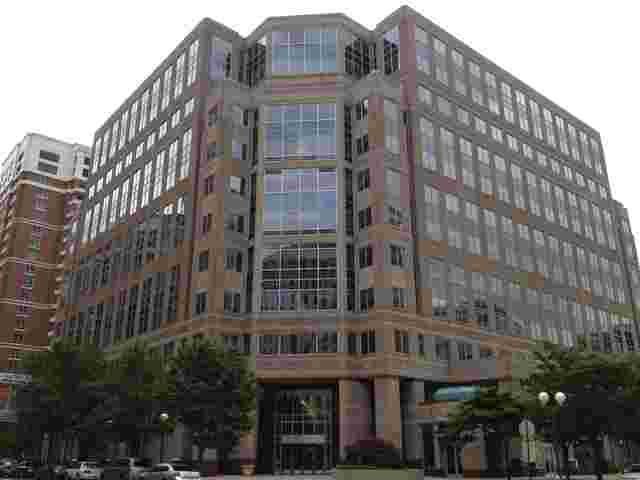
\includegraphics[width=2in]{ch-jpeg/nsf_hq_640x480-q10.jpg} & 
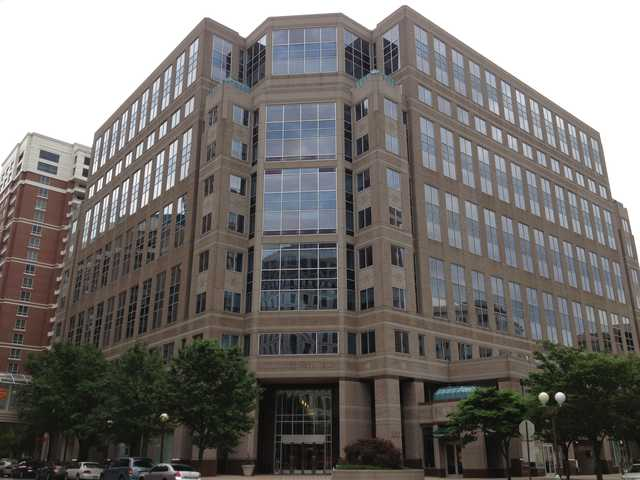
\includegraphics[width=2in]{ch-jpeg/nsf_hq_640x480-q50.jpg} &
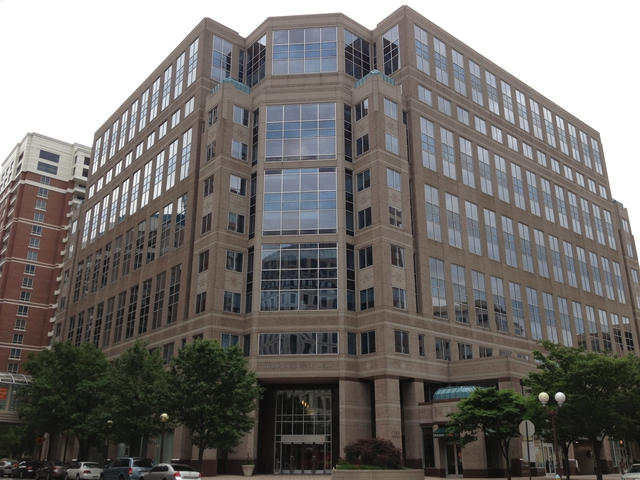
\includegraphics[width=2in]{ch-jpeg/nsf_hq_640x480-q100.jpg} \\
Quality 10 & Quality 50 & Quality 100 \\
23,422 Bytes & 49,305 Bytes & 248,279 bytes \\
1:40 compression & 1:18 compression & 1:4 compression\\
\end{tabular}
\caption{A test image showing three JPEG compression rates. Each image
  is 640x480 pixels. The original uncompressed image required 921,600 bytes.}
\end{figure}

The JPEG file itself is structured as a series of \emph{segments} that are
concatenated together. Each segment begins with a \emph{marker}
consisting of a |FFh| followed by a single-byte code and a data payload. Some segments are fixed
length while others variable size. Typically variable-signed markers
are used for image data or variable-length metadata. The marker
types are described in \tabref{tab:jpeg-format}. Exif metadata is stored in the APP2
segment type, which itself contains its own series of tagged
segments. 

% http://stackoverflow.com/questions/2270082/latex-how-do-i-change-the-font-size-of-a-table-column

\begin{table}
\begin{tabularx}{\textwidth}{l>{\tt}l>{\it}clX}
       & \rm Segment &         &      & \\
Abbrev & \rm Marker  & Payload & Name & Comments\\
\hline
\hline
SOI  & FF D8 &        - & Start of Image & Beginning of file \\
\hline
\hline
APP0 & FF E0 &  $>16$   & JFIF APP0                        & \\
\hline
APP1 & FF E1 & variable & APP1                             & Exif Metadata\\
\hline
APP14 & FF EE & variable & APP14 & Copyright Information\\
\hline
APP\it{n} & FF E\it{n}& - & Application specific           & Other extensions; not widely used\\
\hline
\hline
SOF\it{n} & FF C\it{n} & variable & Start of frame \emph{n}& Start of coding-specific information\\
\hline
SOF0 & FF C0 & variable & Start of Frame (Baseline DCT)    & Also specifies the width, height, number of components, and component subsampling. \\
\hline
SOF2 & FF C2 & variable & Start of Frame (Progressive DCT) & Also specifies the width, height, number of components, and component subsampling. \\
\hline
DHT  & FF C4 & variable & Define Huffman Tables(s)         & Huffman tables follow.\\
\hline
\hline
DQT  & FF DB & variable & Define Quantization Table(s)     & Quantization tables follow.\\
\hline
DRI  & FF DD & 2 bytes  & Define Restart Interval          & Specifies interval between RST\emph{n} markers in macroblocks.\\
\hline
SOS  & FF DA & variable & Start of Scan                    & Image data follows, top-to-bottom scan of image. Progressive DCT JPEGs may contain multiple scans.\\
\hline
RST\it{n} & FF D\it{n}& - & Restart                        & Restart specified by DRI marker.\\
\hline
COM & FF FE & variable  & Comment                          &   Contains comment text\\
\hline
EOI & FF D9 & -         & End of Image\\
\hline
\hline
\end{tabularx}
\caption{JPEG marker types, from
  \url{https://en.wikipedia.org/wiki/JPEG} and
  \url{http://de.wikipedia.org/wiki/JPEG_File_Interchange_Format},  with modifications. Note
  that bytes are in hex.}\label{tab:jpeg-format}
\end{table}

One of the challenges in developing file formats is assuring
\emph{backward compatability} so that newer versions of the files will
be readable by old software that hasn't been updated. JPEG's
segment-based file format is designed to allow backward compatibility:
software that doesn't know how to read a particular segment should, in
theory, be able to just skip over it. In order to do this skip the
software needs a way to find the next segment. JPEG provides two
mechanisms. First, the length of variable-length segments is encoded
in the first two bytes after the marker: if the marker begins \texttt{FFh xx
  s1 s2}, \texttt{FF xx} denotes the segment type and the length
is $256 \times \texttt{s1} + \texttt{s2}$. Second, the character |FFh|
denotes the start of a segment; when |FFh| needs to appear in binary
data, the JPEG standard calls for the value to be entered into the
file as the sequence |FFh 00h|.

From this brief introduction to the standard we can see that there are  several places where
data other than image data might be present in a JPEG file:

\begin{enumerate}
\item After the EOI marker
\item Inside Comment segment
\item Inside the Exif metadata segment
\end{enumerate}

\subsection{A program to validate JPEGs}

To find this kind of information we need a program that understands
the JPEG file format. Many such programs exist, but few of them allow
the degree of control that we require here. Therefore we will present
a short program that understands a small amount of the format and use
it to find the examples of the first two above. The Exif format is
rather complicated, however, so we'll use a specialized open source
tool for that one.

\lstinputlisting[caption=A simple Python program for decoding the JPEG file structure,label=jpeg_scan]{ch-jpeg/jpeg_scan.py}

Listing~\ref{jpeg_scan} is a simple python program that understands
the basic structure of the JFIF and Exif file format. The main
function is |validate_jpeg(fn)|, which opens the named file, reads it
into a buffer called |data|, and then loops through the JFIF
segments. The body of this function is the |while| loop, which checks
to make sure that it has a marker (beginning with a |FF|). It
dispenses with the fixed size segments, provides special handling for
the SOS segment (which extends to the end of the file), and then has
handling for the variable-length segments (the program assumes that
any unknown marker is going variable-length). As an example of
handling variable-sized programs the program prints comments.

Following the function is the part of the program that parses
arguments. If one or more files are provided, they are processed. If a directory name is provided, the program iterates
through all subdirectories, looking for a files with extensions ending
in \emph{.jpg} or \emph{.jpeg}. The debug option causes
\emph{validate\_jpeg()} to print the location and codes of all of the segment markers.

Below is an example of the output that this program produces:

\begin{Verbatim}
output
\end{Verbatim}

We ran this program on several hundred thousand files to look for
JPEGs with anomalous contents. The following sections describe some of
what we found.

\subsection{Files that are not JPEGs}

Files that do not begin with the JPEG ``magic number'' of |FF D8|
cannot be JPEGs. In many cases we found files in other image file
formats---most notably PNG and TIFF. Double-clicking one of these
files will will typically cause the program that is registered to
display JPEG images to attempt to display the file; whether or not the
file actually displays depends on the program. 

\subsection{Data at the end of the JPEG}

One place where information can be hidden is after the JPEG's EOI
marker but before the file's end. This approach hides the data because
programs that display JPEGs stop when they encounter the end of the
image.  

Scanning through the images that we've seen with data after the EOI,
we have found:

\begin{itemize}
\item In a JPEG that was copied from a web page, there were fragments
  of the HTML table that surrounded the image.
\item On a series of photos taken with a Nokia Lumia 822 cellular phone,
  there was 32 character hexadecimal string (128 bits).
\item On a photo taken with an HTC Android phone, there was more than
  10 kilobytes of high entropy data.
\end{itemize}


\begin{lstlisting}[caption={A 40-character block of text consisting of
    two dashes, a 128-bit string (32 hexadecimal
    numbers), two more dashes, a carriage return and a line feed were
    found at the end of every photo taken with a Nokia Lumia 822
    cellular phone. Is this a serial number?},label=lumia822]
--5D9144052FC54aa482D8595FB8D52F1D--
\end{lstlisting}

\subsection{Data in the JPEG Comment}

The JPEG COM Marker introduces comment text that may be up to 64KiB in
length. We analyzed comments on discovered:

\begin{itemize}
\item Many JPEGs had comments indicating the programs that had created
  them. 
\item Apple's iPhoto application sets the Comment to be the same as
  the caption when a slideshow is created.
\end{itemize}

For example, many programs created with the The Gnome Image Manipulation
Program (The GIMP) had comments indicating ``Created with the
GIMP''. It turns out that The GIMP sets this field by default, but it
is only evident when the ``Advanced'' settings of the ``Export'' panel
are exposed.

Comments that reveal the program used to create the image make it
possible to link together multiple images that came from the same
person (although the linkage is unreliable and easily forged). Because
comments may not be removed if an image is edited, they may cause
information to be leaked from one use of a photo to another. 

\sgraphic{ch-jpeg/gimp_save_as}{The GIMP allows the user to specify
  the Comment of a JPEG''}

It turns out that there are several different ways to crop JPEG
photographs on the Macintosh computer that was used to make
\figref{ch-1/nsf_hq}. One of the programs is Apple's iPhoto, which has
check boxes for including ``Title and keywords'' and ``Location
information'' on its export dialog box. 

\bifigure{ch-1/export}{ch-1/export1}{Apple's iPhoto (left) allows the user to select whether or not
  titles and location metadata will be included in exported
  photographs; Apple's Preview tool (right) copies metadata without
  warning the user.}



\section{Exif metadata}\label{sec:exif}
By far the most revealing kinds of information is 

\subsection{Thumbnails}
\subsection{GPS Coordinates}
\subsection{Date and Time}
\subsection{Other Exif Information}

\section{Non-obvious image content information}
\subsection{Non-Subject Information Leakage}
\subsection{Reflections}
\subsection{Details in Shadows}
\subsection{High-Resolution Information}



  \chapter{Private Data in PDFs}

In \chapref{ch:introduction} we recounted a case in which the UK
Parliament inadvertently posted a PDF on a website containing
sensitive information about nuclear subs. But this is hardly a lone
incident. PDFs have been responsible for many kinds of privacy leaks
since the format was introduced by Adobe in 1983

\section{The PDF Format}

Adobe created PDF in the 1990s as a format that would allow computer
users to view and print electronic documents. PDF was designed as a
single electronic container that could be distributed, viewed, and
printed on practically any modern computer system without the need to
install  software or fonts other than a general purpose PDF
reader. Adobe released programs for making and reading PDFs,
originally called Acrobat Distiller and Acrobat Reader, but it also
published the format specification and licensed the patents required
to implement it. Today there are numerous programs that can create,
display and even edit PDF files, and the format has been adopted as an
international standard (ISO 32000-1:2008)\cite{ISO32000-1:2008}.

% \subsection{Before PDF: PostScript}
% 
% Before PDF, electronic documents were typically distributed either as text
% files, such as the Internet RFCs, or as PostScript
% files. \emph{PostScript} is a programming language that Adobe Systems
% created in the 1980s. The key idea 
% of PostScript was that the language was interpreted by the printer, rather than 
% the computer. This allowed relatively small amounts of data to be sent to
% the printer, which would then render the page at the highest resolution
% the device supported. But it also meant that the computer would be
% freed from having to have drives for every different kind of printer
% that might ever be on the market.
% 
% Listing~\ref{hello.ps} below shows a simple PostScript program that draws a
% black box and the words ``Hello World!''  The output of the program
% (shrunk significantly) is shown at quarter size appears in
% \figref{hello-ps-figure}. 
% 
% \lstinputlisting[caption=A simple PostScript program,label=hello-ps-listing]{ch-pdf/hello-ps.ps}
% 
% Even without reading a PostScript manual you
% can draw some conclusions about the programming language simply by 
% inspecting the listing and the resulting output:
% 
% \begin{itemize}
% \item PostScript files begin with the magic number \verb|%!|.
% \item Strings are enclosed in parentheses. 
% \item Font names are preceded with slashes. (In fact, any literal name
%   can be put on the stack by preceding it with a slash.)
% \item Line drawing is performed with human-readable commands like
%   ``moveto'' and ``drawto''. 
% \item Arguments for commands come before the commands themselves,
%   implying that PostScript is a stack-oriented language.
% \item Because sometimes there are line breaks between commands and
%   other times there are not, you can reasonably infer that whitespace
%   is ignored in this file format.
% \end{itemize}
% 
% You can confirm these conclusions and learn more about PostScript by
% reviewing any one of the numerous online PostScript
% tutorial.\footnote{A particularly good online guide is \emph{A First
%     Guide to PostScript} by PJ
%   Weingartner. \url{http://www.tailrecursive.org/postscript/index.html}}
% You can also use a text editor (\S\ref{sec:text-editors}) to enter
% these characters into a file called \emph{hello.ps} and try opening
% the file with a PostScript viewer (\S\ref{sec:postscript-viewer}).
% 
% PostScript's initial use was inside the Apple LaserWriter, the first
% mass-market laser printer. There were inkjet printers, plotters, and
% large-scale laser printers before the LaserWriter, but each had their
% own language. With PostScript, application programs didn't have to
% separately understand how to generate print codes for each
% device. Instead, an application program could simply generate
% PostScript and know that the resulting page would be correctly
% printed. PostScript's most powerful features turned out to be the
% ability to distribute high-quality line art as encapsulated PostScript
% files that could embedded in other documents, scaled, transformed, and
% then printed---all with little work on the part of the application
% program. This, combined with the language's support for high quality
% typography, made PostScript one of the key enabling technologies of
% the 1980's boom in desktop publishing.
% 
% \begin{figure}
% 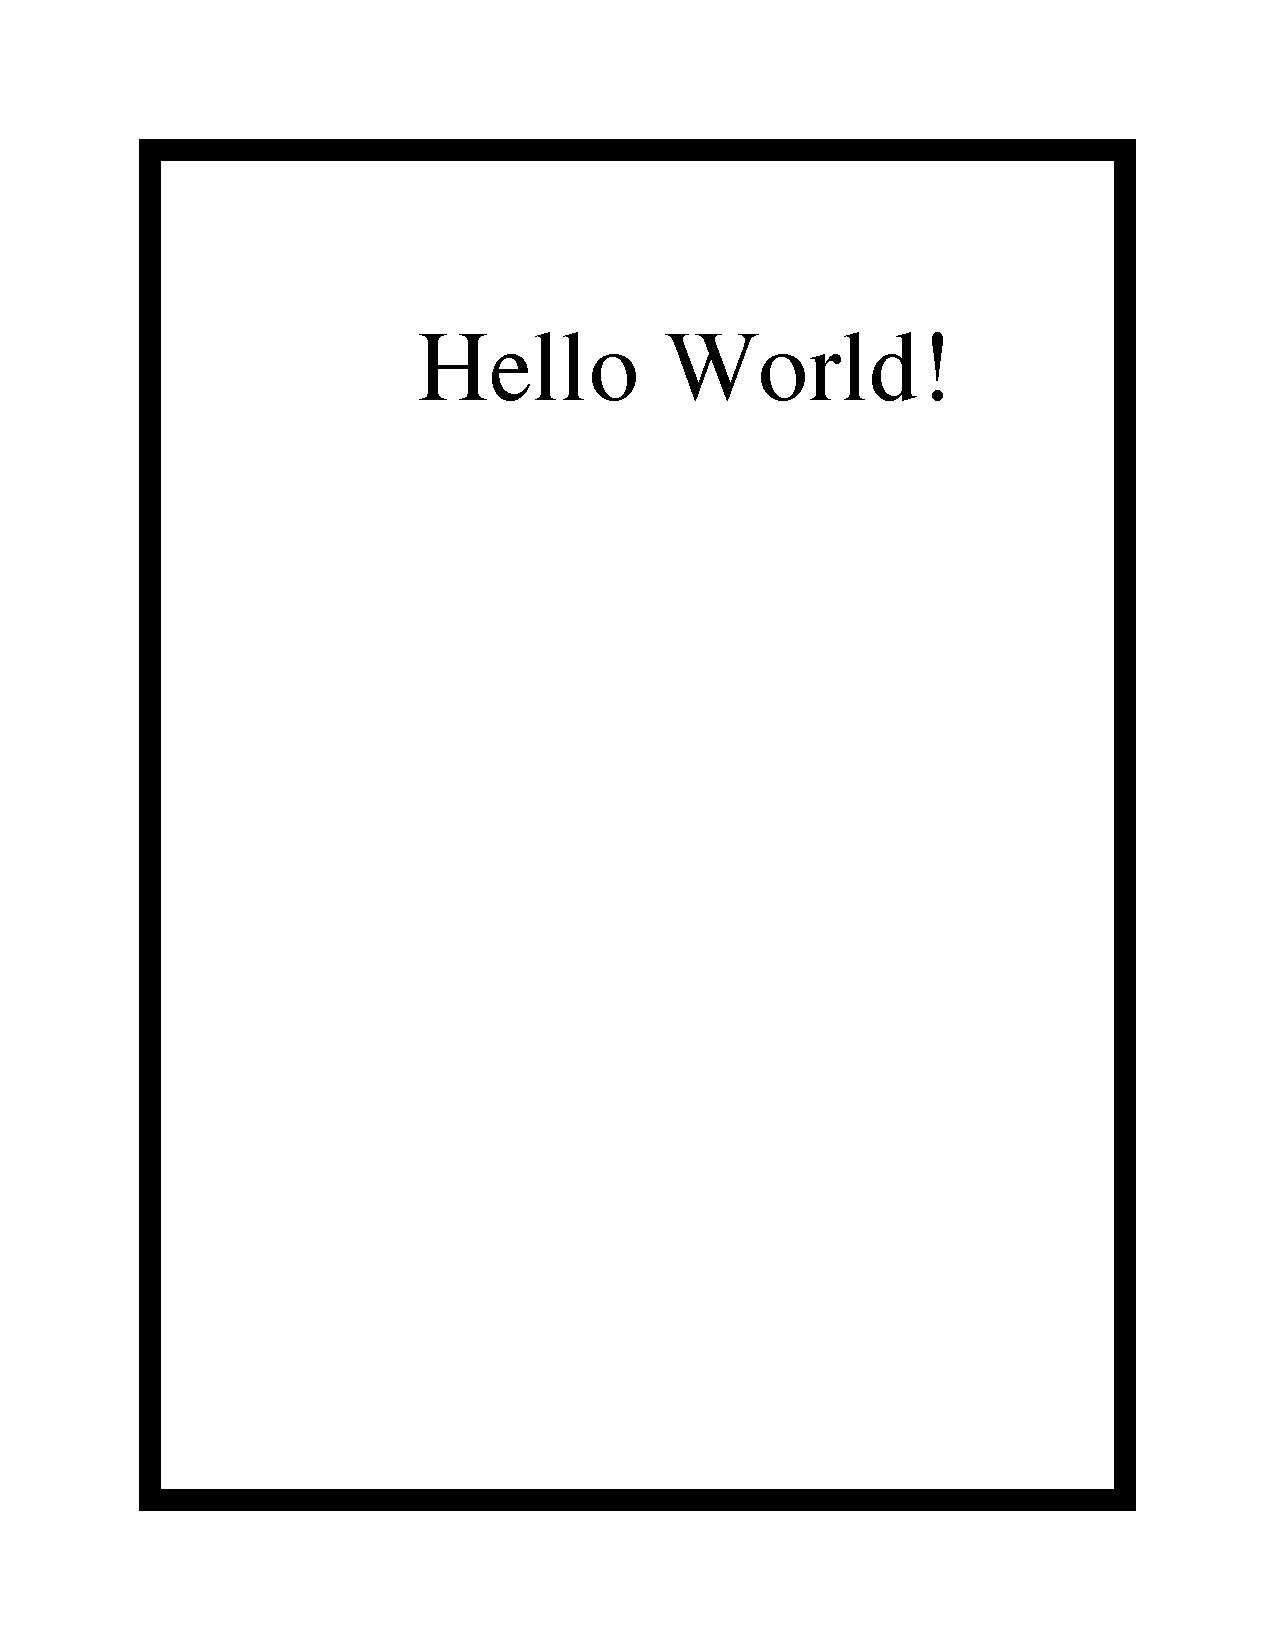
\includegraphics[scale=.25]{ch-pdf/hello-ps.pdf}
% \caption{The output of Listing~\ref{hello-ps-listing}, shrunk to 25\% of
%   the original size.}\label{hello-ps-figure}
% \end{figure}

\subsection{The PDF Specification}

PostScript's power made the language less than ideal as a universal
document format. First, the PostScript is somewhat verbose, so
PostScript files could get quite large. Second, the PostScript
execution context is not reset after each page, with the result that
PostScript viewers could not display pages out-of-order: in order to
show the contents of page 100, the viewer would first need to process
pages 1 through 99. Third, PostScript lacked support for many features
demanded in a modern electronic document format, such as data
encryption, digital rights management, and electronic forms.

The Portable Document Format (PDF) was introduced in 1993 to overcome
these problems with PostScript. Since then, PDF has become an
international standard for distributing born-digital documents, scans
of paper documents, and even electronic forms~ 
PDF was designed as, and as
such it includes direct support for typography, line art and digital
photographs, as well as for document elements such as pagination,
bookmarks and metadata. 

PDF is based on PostScript, but instead of being designed as a general
purpose programming language that produce printed pages, PDF is a
specialized file format. Like PostScript, PDF has
commands for drawing lines, embedding fonts and displaying text. But PDF also has direct support for
document structure; a variety of image and video compression
algorithms; electronic forms; digital rights management; and
cryptography. PDF supports embedded JavaScript for form validation
and other kinds of automation. Any page in a PDF document can be
rendered without reference to any other. 

Listing~\ref{hello-pdf-listing} presents a recast of
Listing~\ref{hello-ps-listing} as a PDF file. Below we summarize some
of the key differences:

\begin{itemize}
\item PDF files consist of a series of numbered objects. 
\item The \verb|moveto| command has been renamed \verb|m|, the
  \verb|lineto| command has been renamed \verb|l|, and so on.
\item At the end of the file a structure (called the cross-reference
  table) which has decimal offsets of the starting point of each object.
\item Finally, there is a trailer that provides information about the
  cross-reference table and the number of the first object required to
  render the document. 
\end{itemize}

Notice that the use of 10-digit decimal numbers means that PDF files
cannot be larger than 9,999,999,999 bytes in size. (Reportedly\footnote{\url{http://forums.adobe.com/thread/1041350}}, there
are additional limits in 32-bit PDF rendering applications.)





PDF gained significant popularity in part because it could be used to 
distribute documents without the  risks of embedded viruses and
privacy-leaking metadata, and because PDF files could not be readily
modified after they were produced and distributed. But as PDF's popularity grew, additional
features were added to both the standard and Adobe's PDF Acrobat
reader. Today PDF can hold arbitrary files as attachments, PDF can
contain JavaScript programs, and PDF can hold significant amounts of
metadata. PDF files can also be edited with a wide variety of
programs, including the open source InkScape program.


If you want to understand the internal PDF specification, you will have a much
easier time reading one of the earlier manuals than the later ones:

\begin{tabular}{lll}
Version & Year & Pages \\
\hline
PDF 1.2 & 1996 & 396 \\
PDF 1.3 (second edition) & 2000 & 696 \\
PDF 1.7 (part 1) & 2008 & 756\\
\end{tabular}



\section{Improperly redacted data}
\section{High-resolution JPEGs}
\section{High-resolution line drawing}
medical information leakage.
\section{Metadata}
\section{References}

\bibentry{nsa-pdfs}



  \chapter{Office Files}

  \chapter{Database Files}

\fi
\ifpartthree
  \bookpart{Working with Storage}
  \chapter{Finding Hidden Data in File Systems}\label{ch-fshidden}

* Alternative data streams

* 

\section{File Deletion and Deleted File Recovery}\label{deleted_file_recovery}
Different file system implementations delete files in different ways.

Traditionally, file systems simply \emph{unlinked} files---the pointer
to the file was removed from the directory, and the blocks associated
with the file were returned to the free list.


\section{Exploiting File System Metadata}
File system metadata can be used to determine usage. 
\cite{dfrws2011:JonathanGrier}

\section{Opportunities for hiding data in File Systems}

Information can be hidden in a file system by storing data in blocks
that are allocated but not used to hold content\cite{dfrws2005:KnutEcksteinAndMarkoJahnke}. 

\begin{Verbatim}
GGRIII: Also, e.g., bmap, under Linux and similar slack space--based techniques on NTFS.
\end{Verbatim}

  \chapter{Carving: Finding Hidden Files in Bulk Data}

\emph{File carving}, sometimes called \emph{data carving} or simply \emph{carving}, is a digital forensics technique used to recover files, file fragments, or other kinds of objects from an input, based on their structure or content, rather than metadata.  The input is most commonly one or more disk images, but can also include other data streams, such as physical memory images or network packet captures. In addition to recovering objects, carving can also be used to simply learn the locations of potentially recoverable objects without incurring the overhead of recovery.  File carving is a powerful tool for recovering data when filesystem metadata (e.g., directory structures) is corrupt or destroyed, which occurs when old files have been deleted or the data source is corrupted, e.g., if data is being recovered from a damaged hard drive.  When file carving is applied to traditional non-volatile storage media, such as hard drives, solid state drives, or removable media such as USB thumbdrives, the objects to be recovered are usually documents (e.g., Microsoft Word or PDF files), images (e.g., JPEG or PNG-format graphics files), video files (e.g., AVI or MPEG format movies), or other common file types.  For physical memory carving, recovered objects are generally operating systems kernel or application data structures, which reveal the current or historical state of a computer system.  

Historically, file carvers operated by looking for file headers and footers, which are unique strings of bytes that appear at predictable places near the beginning and end of files of a particular type \cite{Foremost, Scalpel}.  They may also scan for "milestones", which are other strings of bytes that intervene between the beginning and end of the file, to attempt to eliminate false positives (\emph{do we need to define terms like this here or has this occurred somewhere else?}).  Carving programs often have an option to look for headers only at or near sector boundaries, because new files are always created on a sector boundary.  However, searching the entire input without regard to sector boundaries can enable discovery of embedded files, such as JPEGs embedded in Microsoft Word or other compound document types.  Depending on the circumstances, this may be either an advantage or disadvantage.  

While header/footer--based file carving is still widely used to recover data from storage media, other carving strategies have been developed, to increase the accuracy of file carving tools by incorporating detailed knowledge of specific file types and validation mechanisms, and to expand the scope of carving to other types of media.  Recent research has also concentrated on improving the performance of carving tools and whereas carving was once a fairly time--intensive process, data recovery using carving can now generally be performed at the rate that the target storage media can transfer data.  There has also been some limited success in developing tools that can handle fragmented objects, but these are generally limited to recovery of specific file types and the majority of carving tools cannot automatically reconstruct arbitrarily fragmented objects.   

Applications of file carving and more details about the various file carving techniques currently in use are presented below.

\section{Applications of Carving}

Carving is typically used to recover objects or object fragments (most commonly, files or file fragments) that have been deleted.  Carving might be carried out to support a digital forensics investigation, in the context of criminal or civil litigation, during incident response, or to recover data that's been inadvertently lost, e.g., as a result of  corrupted media or user error.  For the purposes of privacy auditing, carving can be used in precisely the same manner it would be used in a digital forensics investigation of broad scope--namely, to determine what sensitive data can be recovered from target media.  For example, most modern operating systems delete files by simply modify filesystem metadata to make the files "disappear", without actually scrubbing the data blocks previously allocated to the file.  These data blocks "float" in the unallocated regions of storage media, inaccessible to users, until they are allocated to new files and overwritten.  There are numerous situations where this shallow file deletion process exposes sensitive user data to recovery.  For example, when users clear web browser caches, empty the recycle bin on Microsoft Windows systems, clear system logs, or delete files from the command line, typical users lose \emph{control} over potentially sensitive data, but the data is often easily recovered with carving techniques.  

MENTION SWAP SPACE JAIL, OTHER THINGS THAT MAKE DATA PERSIST, BUT ALSO JUST MENTION THAT IT PERSISTS ANYWAY   

Given that carving can recover data that is otherwise completely inaccessible to non-technical users, it is imperative that privacy advocates understand the capabilities and limitations of this forensic technique.  

\begin{Verbatim}


NEED SOME DIAGRAMS THROUGHOUT TO ILLUSTRATE--e.g., I have some 
diagrams that can be adapted which show what happens when a thumb drive is
repeatedly formatted, and what's still recoverable via file carving.
\end{Verbatim}

\section{Header/Footer\-Based Carving}

Header/footer based carving tools use a database of carving rules, with each rule defining how objects of a particular type should be identified in a data stream.  The goal is to identify the starting and ending locations of files in the disk images using these rules and to copy sequences of bytes between the header and footer into regular files for examination.  A rule typically defines a header and optionally, a footer, each of which is a binary string expected to be discovered near the beginning/end of objects of the corresponding type.  For example, for JPEG file types, the appropriate header is 0xFFD8FFE00010 and the footer is 0xFFD9.  The rule also commonly provides other guidance to the carving tool, including the minimum and maximum sizes of matching objects that should be carved, whether alphabetic components of the header and footer are case sensitive, and whether carving operations for an object should cease if the header of a matching object is encountered (this identifies objects stored "back to back" on the storage media).  Other guidance to the carving tool might include whether to choose the footer closest to a discovered header or farthest away from the header, and whether the footer should actually be included in the recovered object.  To illustrate some of these issues, consider the following carving rules from a configuration file for Scalpel, a popular header/footer--based file carver:

{
% SLG commented out \medium, as it caused a problem
% \medium
\begin{Verbatim}
  # image files: GIF, JPG, PNG
  gif  y   100:500000   \x47\x49\x46\x38\x39\x61 \x00\x00\x3b
  jpg  y   1000:8000000 \xff\xd8\xff\xe0\x00\x10  \xff\xd9
  png  y  1000:5000000  \x50\x4e\x47?  \xff\xfc\xfd\xfe
  #
  # Legacy Microsoft Office documents
  doc  y  1000000      \xd0\xcf\x11\xe0\xa1\xb1\x1a\xe1\x00\x00 
  # Illustration of regular expression-based headers and footers
  xyz  y   100000  /GGG[^G]/    /[0-9]HHHHH/
\end{Verbatim}
}

Comments in the example above begin with a hash mark ("\#") and are ignored by the carving tool.  The first rule carves GIF format images files, and used "gif" as the extension for recovered files.  The "y" indicates that the header and footer and are case-sensitive.  "100:500000" indicates that only files between 100 and 500,000 bytes (inclusive) should be recovered.  The final two elements of the rule are the header and footer, represented by hexadecimal strings.  The JPEG and PNG rules are similar.  The Microsoft Office rule is different, in that no footer is specified.  In this case, files that match the header are carved to the maximum size specified (in this case, 1,000,000 bytes).  Rules like this are wasteful of space, but if file types don't have strings that can be reliably predicted to be near the end of file, then for header/footer--based carving, there's essentially no choice.  The final rule illustrates header/footer--based carving being used to carve objects with headers and footers specified by regular expressions.  In this rule, files of a maximum of 100,000 bytes are carved if they begin with a string of three "G" characters, followed by a character other than a "G".   The file is terminated by a digit (0--9) followed by five "H" characters.  Using regular expressions for headers and footers potentially decreases performance of the carving tool, but provides a much more powerful means to describe the objects to be recovered.  Creating a new rule can be time--consuming, because some knowledge about the common structure of files of the new type is required, but this knowledge need not be nearly as deep as for \emph{semantic carving}, covered later in the chapter.

One benefit of header/footer-based carvers is that they can retrieve files from a raw disk image in a filesystem--agnostic way, operating regardless of the type of filesystem on the disk image.  Perhaps more importantly, file carving is possible even if the filesystem metadata has been destroyed, such as during a filesystem format operation or as a result of file corruption due to media damage, a power outage, or similar event.    One limitation of header/footer--based carving tools is that an object's data must be contiguous to be carved properly.  With manual intervention or multiple carving steps which prune out previously recovered objects from the target media, some non-contiguous objects can be recovered, but in general fragmented objects are problematic.  Still, header/footer--based carvers that encounter fragmented objects can still partially recover the objects, and even object fragments may pose significant risks to privacy (\emph{probably some examples here}). 

\section{Carving with Validation}



\section{Semantic \/ Deep Carving}

\begin{Verbatim}

There's some ambiguity regarding what to call file\-structure aware carving. 
I like "semantic carving". We could also use "file structure aware carving" 
from the taxonomy on the Wiki but this sounds so clumsy.

Talk about photorec and others here

Detailed knowledge of internal structures of files greatly increases accuracy
when carving pristine files, but it's time consuming to accommodate new file
types (hacking required, lots of error conditions in the parser that must be 
dealt with), documentation for new file types may not be generally available, 
mild corruption in file may result in the file being dismissed as not matching
(bad, because partially recovered objects can still be very invasive of privacy
and are often useful in investigative scenarios)

\end{Verbatim}

\section{Carving Fragmented Files}

Dealing with fragmented objects is the most difficult problem in carving.  In legacy filesystems such as FAT, which does not incorporate strategies to reduce file fragmentation, many small files are likely to be stored contiguously, because files are created on cluster boundaries and cluster sizes under FAT tend to be rather large.  Larger files on FAT filesystems, however, are commonly fragmented\cite{dfrws2007:SimsonLGarfinkel}.  While modern filesystems such as NTFS, ext2/3/4 and HFS+ do take steps to ensure that fragmentation of files is reduced, fragmentation does still occur.  Furthermore, performance for SSDs does not benefit from legacy anti--fragmentation mechanisms, and some of these mechanisms may actually reduce SSD lifespan.  As a result, some anti--fragmentation strategies are suppressed when SSDs are in use.  

\begin{Verbatim}
Do we want to get into the anti-fragmentation stuff in e.g., ext2/3/4 and 
HFS+?
\end{Verbatim}

\begin{Verbatim}
Digital Assembly: Download new trial and check it out.  Wasn't so impressive last
time I looked at it.
\end{Verbatim}

\section{Memory Carving}

\begin{Verbatim}
Physical memory acquisition, Volatility, maybe specialized, standalone stuff, but
most of that functionality is making its way into Volatility anyway
\end{Verbatim}

\fi
\ifpartfour
  \bookpart{Network Analysis}
  \chapter{Capturing Network Traffic}

  \chapter{Privacy Leaks in the Web}
Cookies and web bugs.

Facebook Twitter

- How personal information gets embedded as people communicate over the cloud.

\section{Web Analytics}


  \chapter{Email Analysis}

\section{webmail vs. client mail}

\section{Reading Email headers; header: blue / yellow}
- show where email header comes from

 - Show how email pics up headers as it moves through the system

Email bugs  (DNS)

Email redirecitons



\fi
%\ifpartfive{
%  \bookpart{Advanced Topics}
%  \chapter{Encryption}\label{ch:encryption}
\section{Encrypting File Systems}
\section{Network Encryption}
\section{Key Management}

%  \chapter{Memory Analysis}\label{ch:ram}
\subsection{Memory Parsing}

The memory of a desktop, laptop or cell phone is a mosaic of 4096-byte
blocks that variously 
contain running program code,  fragments of programs
that recently ran and have exited, portions of the computer's
operating system, fragments of what was sent and received over the
network, fragments of windows displayed on the computer's screen, the
computer's copy-and-paste buffer, and other kinds of information. Memory
changes rapidly---typical memory systems support several billion
changes per second---so it is nearly impossible to make a copy that is
internally consistent without halting the machine. An added complication is that the very
specific manner that programs store information in memory is rarely
documented and changes between one version of a program and
another. As a result, each version may need to be painstakingly reverse-engineered by
computer forensics researchers. Thus, memory analysis is time consuming, very
difficult, and necessarily incomplete.

Despite these challenges, recent years has seen the development of
forensically sound techniques for acquiring and analyzing the contents
of a running computer system. Today there are both open source and
proprietary memory analysis tools. These tools can take a memory dump
and report the system time when the memory was captured, display a
list of running processes, open files, and even display the contents
of the computer's clipboard and screen. Today memory analysis tools
are widely used for reverse-engineering computer viruses, worms and
other kinds of \emph{malware}, as well as for understanding an
attacker's actions in computer intrusion cases. Memory analysis can be combined
with carving to recover digital photographs and video.



\section{Acquiring RAM}
\section{Analyzing RAM with volatility}

%\fi
\ifpartsix{
  \appendix
  \bookpart{Appendices}
  \chapter{Designing a good forensics experiment}

This chapter explores what is involved in creating a good computer
forensics experiment.

\section{Why experiment?}

why should you experiment?

\section{What is the purpose of the experiment? - what you can provide and what you can't}
\section{Start with a wipe}
\section{Use Self-Identifying Data}

What self-identifing data is.


% M-sequences in radar
% KW37 - keying is for a day; you can join anytime.
% Watermarking - covert and robust go together
% hackmem search algorithm

\section{Sampling vs. Complete Analysis}

sometimes you can analyze all the data, but frequently you can't

\section{Error Rates}
\subsection{What is an error rate}
\subsection{Error rates from hardware}
\subsection{Error rates from sampling}
         % Designing a DF experiment
  \chapter{Glossary}
\begin{description}
\item[Allocated (files and sectors)] Allocated files are files that can be viewed through
  the operating system; allocated blocks are blocks that have been
  allocated to a specific file and will not be re-used by the
  operating system unless the contents are first relocated
  elsewhere. cf with \emph{deleted files}.
\item[Bit] A binary digit (0 or 1). The word ``bit'' was coined by
  John W.\ Turkey (1915-2000) while working at Bell Labs and first appeared in
  print in Claude Shannon's seminal 1948 article on information
  theory, \emph{A Mathematical Theory of Communication}. (Turkey also
  coined the word \emph{software}.) Abbreviated with a lower-case
  letter \emph{b}.
\item[Byte] An ordered set of bits used to represent the minimum
  amount of data that can be read or written to a computer memory at a
  time. Modern computers use 8-bit bytes, allowing for 256
  ($2^8$)possible values (typically 0 through 255 if the byte is
  interpreted as an unsigned number, or -128 through 127 if the byte
  is interpreted as a signed value.) Abbreviated with an upper-case
  letter \emph{B}.
\item[Compression] A mathematical process for reducing the size of a
  file or other digital object. Compression can be \emph{lossless} or
  \emph{lossy}. In Lossless compression the original file can be recovered by
  \emph{decompressing}, while with lossy compression information is
  lost and the exact original cannot be recovered. (However, lossless
  compression may have such high fidelity that a human being is unable
  to distinguish between the original and the decompressed objects.
\item[Deleted files] Files whose contents can be recovered but the
  sectors of which are not allocated.
\item[Digital Forensics] ``A branch of forensic science encompassing the
  recovery of and investigation of material
  found in digital devices, often in relation to computer crime.''\cite{reith:examination}
\item[Digital Trace Evidence] Another name for \emph{residual data}.
\item[Disk Image] A byte-for-byte copy of all the data on hard drive,
  camera card, or other kind of sector-oriented mass storage
  device. Disk images can contain additional metadata such as an
  embedded cryptographic hash of the original media, the date that the
  image was made, the examiner who made the image, as well as notes.
\item[Disk Imager] A program for making disk images.
\item[Media Exploitation] The extraction, translation and
  analysis of digital documents and media to generate
  useful and timely information.
\item[File] An ordered collection of 0 or more bytes. Files have a
  length; they may optionally metadata such one or more file names,
  modification dates, owners, and other information.
\item[File Header] One or more fixed bytes at the beginning of a
  file. For example, ZIP files begin with the file header ``PK'' (hex
  \texttt{50 4B}), while JPEG files begin with the field header
  \texttt{FF D8 FF E0}.
\item[File Footer] One or more fixed bytes at the end of a file. JPEG
  files end with the file footer \texttt{FF D9}.
\item[File System] Part of a computer's operating system which
  controls the storage of files on a mass storage system such as a
  hard drive or camera card.
\item[Forensic Science]
\item[Hash Value] Always say \emph{hash value}, never \emph{hash
  code}, since the word \emph{code} might refer to either the hash
  value or the program that computes the value.
\item[Investigator-Centric] Digital Forensics is said to be
  ``investigator-centric,'' meaning that most of the advances in the
  field have been to serve specific needs of investigators, rather
  than based on what is scientifically or technically possible.
\item[Logical Block Address (LBA)] \emph{Sectors} of a mass storage
  device are arranged in numbered sectors, starting with LBA 0. Early
  PC systems used hard drives that supported a 22-bit LBA and 512-byte sectors, allowing for a
  total of $2^{22}\times 2^{9}=2^{31}=2\textrm{TB}$ of storage. The
  current Advanced Technology Attachment standard, ATA-6, supports
  48-bit LBA addresses and a 4096-bit sector size, for a maximum disk
  with $2^{48}\times 2^{12}=2^{60}\approx 1,152,921\textrm{TB} \approx 1
  \textrm{EB (exabyte)}$ of storage.
\item[magic number]
\item[Malware] Software that embodies evil intent, such as to damage
  computer systems or steal private information. Computer Viruses,
  worms, and Trojan horses are examples of malware. 
\item[Metadata] Data about other data. The created, modified and
  access timestamps associated with a file on a camera card are
  examples of metadata.
\item[MD5] Message Digest \#5, a cryptographic hash algorithm
  developed by MIT professor Ron Rivest in 1991. Although MD5 is
  widely used in computer forensics, MD5 has known flaws and should
  not be used in applications that depend upon collision resistance.
\item[milestones] \pageref{def:milestones}
 \item[Network forensic analysis tool (NFAT)] A system that can record
   packets as they move over a network and perform detailed
  after-the-fact analysis.
 \item[normalization]
 \item[Packet] A set of bytes that are sent over a network. Most
   Internet packets range in size from 40--1500 bytes.
 \item[PCAP File] A packet capture file, which is typically a set of
   packets that were recorded using a packet sniffer.
 \item[Packet sniffer] A program or device that can record packets are
   they move over a network.
 \item[Packet Traces]
 \item[Provenance]
\item[Preview] an application on Apple Macintosh for viewing images
  and PDF files. 
\item[Residual Data] data that is left behind on a computer after an
  operation is completed but is no longer in active use. For example,
  most computer systems erase the file name when a file is deleted,
  but do not overwrite the actual file contents. These contents remain
  on the drive as residual data, recoverable with computer forensic tools.
\item[Sector] The minimum amount of data that can be read or written
  to a mass storage device. Modern hard drives use sectors of 4096
  bytes; drives with 512-byte sectors have been common since the mid
  1970s and are still widely used today.
\item[Subject Computer and Data] The computer system and data that are
  being analyzed as part of a digital investigation. This may be data
  extracted from a computer belonging to a suspect in a crime, but it
  may also be data from the computer of a victim. Subject data may
  even be data generated during the course of a DF tool.
\item[Subject] is a common shorthand for the owner or primary use of a computer
  system from which subject data was obtained. 
\item[Tool-Based] Digital Forensics is said to be ``tool-based,''
  meaning that most investigators in their investigations to the
  capabilities provided by today's tools---investigators generally do
  not devise their own digital experiments or invent new approaches
  for working with data to solve specific cases.
\item[Timestamp]
\item[Unallocated sectors] Sectors that are not allocated to files or
  metadata, but are instead available for use by the file system
\end{description}

  \chapter{Open Source Forensic Tools}

\section{Sleuth Kit}

Sleuth Kit is an open source digital forensics toolkit for extracting
files from disk images. Sleuth Kit understands a variety of disk image
formats, partitioning schemes, and file systems. With Sleuth Kit, you can can recover
both allocated files and files that have been deleted directly from a
disk image, without having to ``mount'' the disk image by the host
operating system. An added advantage of Sleuth Kit is that it runs on
Windows, Linux, and Macintosh systems, allowing you to access data
from disk images even if your underlying operating system does not
understand the format.

The Sleuth Kit website\footnote{http://sleuthkit.org} has information
on Sleuth Kit, Autopsy (a graphical interface for SleuthKit), the
Sleuth Kit Hadoop Framework (for processing large numbers of hard
drives in a cloud computing environment), and other tools. 
Precompiled binaries for

\subsection{Sleuth Kit under Windows}
Windows users should download pre-compiled Sleuth Kit binaries from Source
Forge.\footnote{\url{http://sourceforge.net/projects/sleuthkit/files/sleuthkit/4.0.2/}}
and install them in into |c:\sleuthkit|.

\subsection{Sleuth Kit under Linux}

\subsection{Sleuth Kit under Macintosh}

\section{Network Monitoring with WireShark and tcpflow}

\subsection{WireShark and tcpflow on Windows}
\subsection{WireShark and tcpflow on Linux}
\subsection{WireShark and tcpflow on Macintosh}

\section{Bulk Data Analysis with Bulk Extractor}

\subsubsection{Bulk Extractor on Windows}
\subsubsection{Bulk Extractor on Linux}
\subsubsection{Bulk Extractor on Macintosh}

\sgraphic{ch-1/windows-console}{Setting your Windows console for 132
  rows of text and 9999 lines of scrollback will improve the usability
  of many text-based commands.}

\section{Text Editors}\label{sec:text-editors}

\section{PostScript and PDF Viewers}


\section{Making Hex Dumps}

Notepad++ / Install a hex editor plugin

\subsection{Linux}
On Linux systems you may need to explicitly install Python 3. Do so on
Fedora by typing:

\begin{code}
$ (@ \hl{sudo yum install python3} @) 
\end{code} 
% $

\subsubsection{Hex Dumps under Linux (Fedora)}

Popular tools for creating hex dumps on Linux include \texttt{od}
(octal dump) and \texttt{xxd}.  The \texttt{od} is part of the base
release. xxd must be installed from the package
\texttt{vim-common} with the yum command:

\begin{code}
$ (@ \hl{sudo yum install vim-common} @)
\end{code}

Note: We're not sure why xxd is part of
  vim-common. If you didn't know this, you could could the command
  \texttt{yum whatprovides} to learn which package provides it:
\begin{code}
$ (@ \hl{yum whatprovides xxd} @)
Loaded plugins: langpacks, presto, refresh-packagekit
2:vim-common-7.3.712-1.fc18.x86_64 : The common files needed by any version of the VIM editor
Repo        : fedora
Matched from:
Filename    : /usr/bin/xxd
$
\end{code} 
%$


\section{Hashing}

In computer science a \emph{hash function} is any function that maps a
sequence of zero or more characters (called a \emph{string}) to an
binary number of a specific fixed size---that is, a fixed number of
bits. A 16-bit hash function can produce $2^{16}=65,536$ different hash values, while a
32-bit hash function can produce $2^{32}=4,294,967,296$ possible hash
values. Hash functions are designed so that changing a single
character in the input results in a completely different number. While
the pigeonhole principle guarantees that many different strings will
have the same hash value---something that's called a \emph{hash
  collision}---the more bits in the hash has, the smaller the chance
of a collision.

Hashing was invented by H.\ P.\ Luhn in a 1953 IBM technical memo;
it's been widely used for computerized text processing since the
1960s. For example, because every sentence in a document can be
treated as a string, hashing makes it possible to rapidly see if the
same paragraph ever repeats in a long document: just computer the hash
value for each paragraph, put all of the hashes into a list, sort the
list, and see if any number repeats twice. If there is no repeat, then
no paragraph is repeated. Of course, if a number \emph{does} repeat,
then it's necessary to look at the paragraphs that correspond to those
two numbers to determine if the same paragraph really is repeated
twice or the duplicate is the result of a hash collision. Using hashes
in this manner is much faster than working directly with the
paragraphs because it is much faster for computers to compare numbers
than sequences of words---even when you take into account the time to
perform the hashing.

(Interesting fact: The name \emph{hash} comes from the way hash functions are typically
implemented as a two-step process that first chops and then mixes the
data, much in the way that one might make hash in the kitchen!)

In 1979 Stanford University PhD student Ralph Merkle invented a way to use
hashing for computer security\citep{merkle:79}. Merkle's idea was to
use a hash
function that produced more than 100 bits of output and that
additionally had the property of being \emph{one-way}. That is, it was
a function for which it was relatively easy to compute the hash of a
string, but it was nearly impossible, given a hash, to find a
corresponding string. The essence of Merkle's idea was to use a
document's 100-bit one-way hash as a stand-in for the document itself
for certain mathematical purposes. For example, instead of digitally
certifying a 50-page document, the document could be reduced to a
100-bit hash and the hash could then be certified. Because there are so many different possible hash values
($2^{100}\approx10^{30}$), Merkle reasoned that it would not be
possible for an attacker to take the digital signature from one document and use it
to certify a second document---because to do so would require that
both documents had the same hash value.

Today digital signatures applied to hashes are
the basis of many cyber security system. Digital signatures protect
credit card numbers sent over the Internet, certify the authenticity
and integrity of code run on iPhones, and validate keys used play
digital music. The idea of hashing has been applied to other areas as
well---in particular, forensics.

One of the first and continuing uses of hashing in DF was to establish
\emph{chain-of-custody} for forensic data. Instead of hashing a
document or a file, the hash function is applied to the entire disk
image---that is, \emph{all} of the bytes extracted from a hard
drive. Many law enforcement organizations will create two
disk images of a drive and then computer the hash of each image.  If the values match, then the
copies are assumed to each be a true copy of the data that were on the
drive. The hash value is then included in the official report. With
the hash recorded, the image file can be copied to a server at the
police department, to an investigator's workstation, or even given to
a forensic expert working for the other side. Any investigator with the
data can calculate the hash and see if it matches the original
reported value. If the hashes match, the investigator can be sure that
not a single bit in the disk image has been changed since the original
image was recorded. Hashing is so important that many DF tools can
automatically validate an evidence file by recomputing the hash and
comparing it with a stored value.

A second use for hashing is to identify specific
files. This approach takes advantage of the property that it is
extraordinarily unlikely for two files to have the same
hash value. File hashes can thus be used to identify files in much the
same way that a person can be identified by their fingerprints. 

Today forensic practitioners distribute databases containing the file
hashes as a standard part of forensic processing. The best known of these data
sets is the National Software Reference Library Reference Data Set,
distributed by the National Institute of Standards and
Technology\cite{nist-nsrl-rds-march2012}. These data sets can be used
to identify \emph{known goods}, such as programs distributed as part
of operating systems, or \emph{known bads} such as computer viruses,
stolen documents and child of pornography. Recent work is now
applying cryptographic hashing to blocks of data smaller than
files\cite{garfinkel:sector-id}, taking advantage of the fact that
even relatively short 512-byte and 4096-byte segments taken from
files can be highly identifying. 

File and sector identification with hashing means that a hard drive
containing millions of files can be automatically searched against a
database containing the hashes of hundreds of millions of file hashes
in a relatively short amount of time---perhaps just a few hours. Importantly, the search can be done without any human
intervention.




  \section{Python}
This book makes extensive use of the Python programming language for
its examples. All of the examples are tested under Python~3.3,
although Python~2.7 may work with most of the demonstration programs
as well.  This section describes specific aspects of the Python
programming language that are important in our examples and that may
be missed in an introductory Python programming class.

\subsection{Reading and Writing Files: Binary vs.\ Text}

When a Python program opens a file that file may be opened in one of
two modes: \emph{text} or \emph{binary}.  When opened as text, Python
assumes that the files contain text characters that have been encoded
with an appropriate codec---for example, that they are Unicode files
coded as UTF-8. Assuming such a codec qcan cause problems when reading
binary data, since many binary combinations do not represent valid
characters. To avoid this problem, files will normally be opened in
binary mode. This is done by opening files with method
|open(filename,"rb")|.

\subsection{Python's struct.unpack}
Much of the information on computers is stored as binary encoded
values. Such values can be easily read and written using python's
|struct.unpack| method, which reads a binary structure and returns a
python tuple of the decoded values.  

The binary structure is decoded using a \emph{format
  specification}. For example, this Python fragment will print the
decimal value of the hex string DEADBEEFh:

\lstinputlisting[caption=A program to print the decimal value of the hexadecimal number \texttt{DEADBEEFh}]{ch-1/deadbeef.py}


\subsection{Path Delimiter}
Windows uses the backslash (|\|) as a path delimiter, while Unix
systems use the forward slash (|/|). In general this is not a problem,
because Python run on Windows will treat either slash as a path
delimiter. So in general, this book will use the forward slash as a
path delimiter, even for code that runs on Windows-based computers.

\subsection{Accessing Raw Devices}

A ``raw'' device is a device file that can be opened by user programs
like a normal file but reads and writes are sent directly to the
underlying physical device. Typically access to the raw disk devices 
requires administrative privileges, since access to the raw device
bypasses the computer's operating system.

To access the physical drives on a Windows computer open the hidden
physical drives |\\.\PhysicalDrive0| through
|\\.\PhysicalDriveNN|. To open the physical drive for reading use use
mode |rb|, for writing use the ``updating'' mode |rb+|. List the
physical drives on your Windows system with the command:

\begin{code}
c:\ (@ \hl{wmic diskdrive list brief /format:list} @)
\end{code}

Unix-based systems associate two pseudo-files in the |/dev/| directory with
each physical device; additional pseudo-files map to disk
partitions. Macs use |/dev/diskNN| for block devices and
|/dev/rdiskNN| for raw devices. Partitions are identified by appending
a |sJ|, where |J| is the partition number.  List the physical drives
on a Mac with the command:

\begin{code}
$ (@ \hl{ls -l /dev/disk*} @)
\end{code}
%$

Linux systems name block devices |/dev/sdA| where |A| is a letter |a|
through the highest device letter; partitions are identified with an
appended letter. Modern Linux systems also map physical devices in
additional locations, including the directory |/dev/disk/by-uuid/| for
a list of drives by UUID, |/dev/disk/by-partuuid| for partitions by
UUID, |/dev/disk/by-path| for their location on the PCI or SCSI bus,
and |/dev/disk/by-id| for device IDs. Linux systems may also map
block devices in the |/sys/dev/block/| and character devices in
|/sys/dev/char/|. List the physical drives
on a Mac with the command:

\begin{code}
$ (@ \hl{ls -l /dev/sd*} @)
\end{code}
%$


\subsection{Making Graphs}
There are a large and growing number of producing graphical displays
from Python. This book uses the Python library matplotlib for data
visualization and graphiviz.


\subsection{Python3 on Windows}
Windows users should download the most recent version of Python 3 from
\url{http://www.python.org/getit}. Use the \emph{Windows X86-64 MSI
  Installer} if you have a 64-bit system and a \emph{Windows x86 MSI
  Installer} for 32-bit system. Although the 32-bit version will work
on a 64-bit system, 32-bit programs running on a 64-bit system are
presented with a slightly incorrect view of the computer's file
system, which can be confusing in some instances.\footnote{Microsoft
  uses the term Windows on Windows 64, or WOW64, to describe the
  process of running 32-bit applications on 64 bit Windows. For a
  complete discussion, search for WOW64 on MSDN or Wikipedia.}


On Windows, install matplotlib for Python 3.3 with:

\subsection{Python3 on Linux}
On Linux systems you may need to explicitly install Python 3. Do so on
Fedora by typing:

\begin{code}
$ (@ \hl{sudo yum install python3} @) 
\end{code} 
% $

\subsection{Python3 on Macintosh}
On MacOS, install matplotlib for Python 3.3 with:
\begin{code}
$ (@ \hl{sudo port install py33-matplotlib} @)
\end{code}
%$

\section{Setting Up your Computer}
This section provides recommendations for setting up your computer to
make the most of the examples and exercises in this book. Remember,
these are \emph{recommendations,} not requirements.

\subsection{Windows}
Once you have installed Python, you may wish to modify your Windows
console so that it has 132 rows of text and 9999 lines of
scrollback. You can do this by running the |cmd.exe| program from the
Start menu then right-clicking on the window's titlebar and selecting
the ``Properties'' menu, as shown in \figref{ch-1/windows-console}.

Windows users may also wish to become familiar with the Windows
PowerShell, a replacement for |cmd.exe|.

\sgraphic{ch-1/windows-console}{Setting your Windows console for 132
  rows of text and 9999 lines of scrollback will improve the usability
  of many text-based commands.}

If you do not have a C++ compiler, you should install one. Many
Windows users will feel most comfortable with an integrated
development environment (IDE). We
recommend:

\begin{itemize}
\item Code::Blocks\furl{http://sourceforge.net/projects/codeblocks/},
  a popular Open Source IDE that includes the mingw compiler suite 
\item Orwell Dev-C++
  (\url{http://sourceforge.net/projects/orwelldevcpp/})
\item Visual Studio Express 2012 for Windows
  Desktop\furl{http://www.microsoft.com/visualstudio/eng/products/visual-studio-express-products},
  Microsoft's compiler, allows development in C++, C\# and
  VB.NET. Runs on Windows 7 and later versions.
\end{itemize}

\subsection{Linux}

\subsection{MacOS}

For Mac systems we recommend installing Python 3 with the MacPorts
system. Download MacPorts from \url{http://macports.org/} and then type:

\begin{code}
$ (@ \hl{sudo port install python33} @) 
\end{code} 
% $



  % http://www.scipy.org/Plotting_Tutorial
\chapter{Visualizing Data}
\section{Matplotlib}
<<<<<<< HEAD
\section{Other Options}
\begin{description}
\item[Mayavi] is a 3D Scientific Data Visualization system supporting
  complex interactive graphics. Download it from \url{http://code.enthought.com/projects/mayavi/}
\item[MqthGL] MathGL is a library for producing scientific
  visualizations. It is very fast and can be called from C, C++,
  Python, Qt, FLTK and OpenGL. Unfortunately, it appears to only run
  under Windows and Linux. You can download it from \url{http://mathgl.sourceforge.net/}
\item[PyQwt] provides Python bindings for the Qwt C++ graphing system,
  which creates graphics with Qt. It can create much larger
  visualizations than matplotlib, but it is somewhat more difficult to
  use. \url{http://pyqwt.sourceforge.net/}
\end{description}
=======
\section{JFreeChart}
\section{Storing Data To Visualize}
Javadb
sqlite
flat files

launch4j
>>>>>>> 1b706fb94be23cbd5bd7480d8e240506125854cf

  \chapter{Chunk-Based Container Files}
\section{Introduction - what is a chunk-based file?}
\section{JPEGs}
\section{GIFs}
\section{TAR / RAR}

  \chapter{References}

\section{Books}\label{section:books}
The following books are referenced in this book:

\printbibliography[heading=bibempty,type=book]

\cite{carrier-file-systems}
\section{Articles}


\fi


%%  LocalWords:  ap

%----------------------------------------------------------------------------------------
%	BIBLIOGRAPHY
%----------------------------------------------------------------------------------------

\chapter*{Bibliography}
\addcontentsline{toc}{chapter}{\textcolor{ocre}{Bibliography}}
\section*{Books}
For a list of books, please see page~\vref{section:books}.
% \addcontentsline{toc}{section}{Books}
% \printbibliography[heading=bibempty,type=book]
\section*{Articles}
\addcontentsline{toc}{section}{Articles}
\printbibliography[heading=bibempty,nottype=book]

%----------------------------------------------------------------------------------------
%	INDEX
%----------------------------------------------------------------------------------------

\cleardoublepage
\setlength{\columnsep}{0.75cm}
\addcontentsline{toc}{chapter}{\textcolor{ocre}{Index}}
\printindex

%----------------------------------------------------------------------------------------

\end{document}
